\subsection{Giao diện chương trình}

% \subsubsection{Người dùng khách và xác thực}

\paragraph{Trang chủ khách}

\begin{figure}[H]
\centering
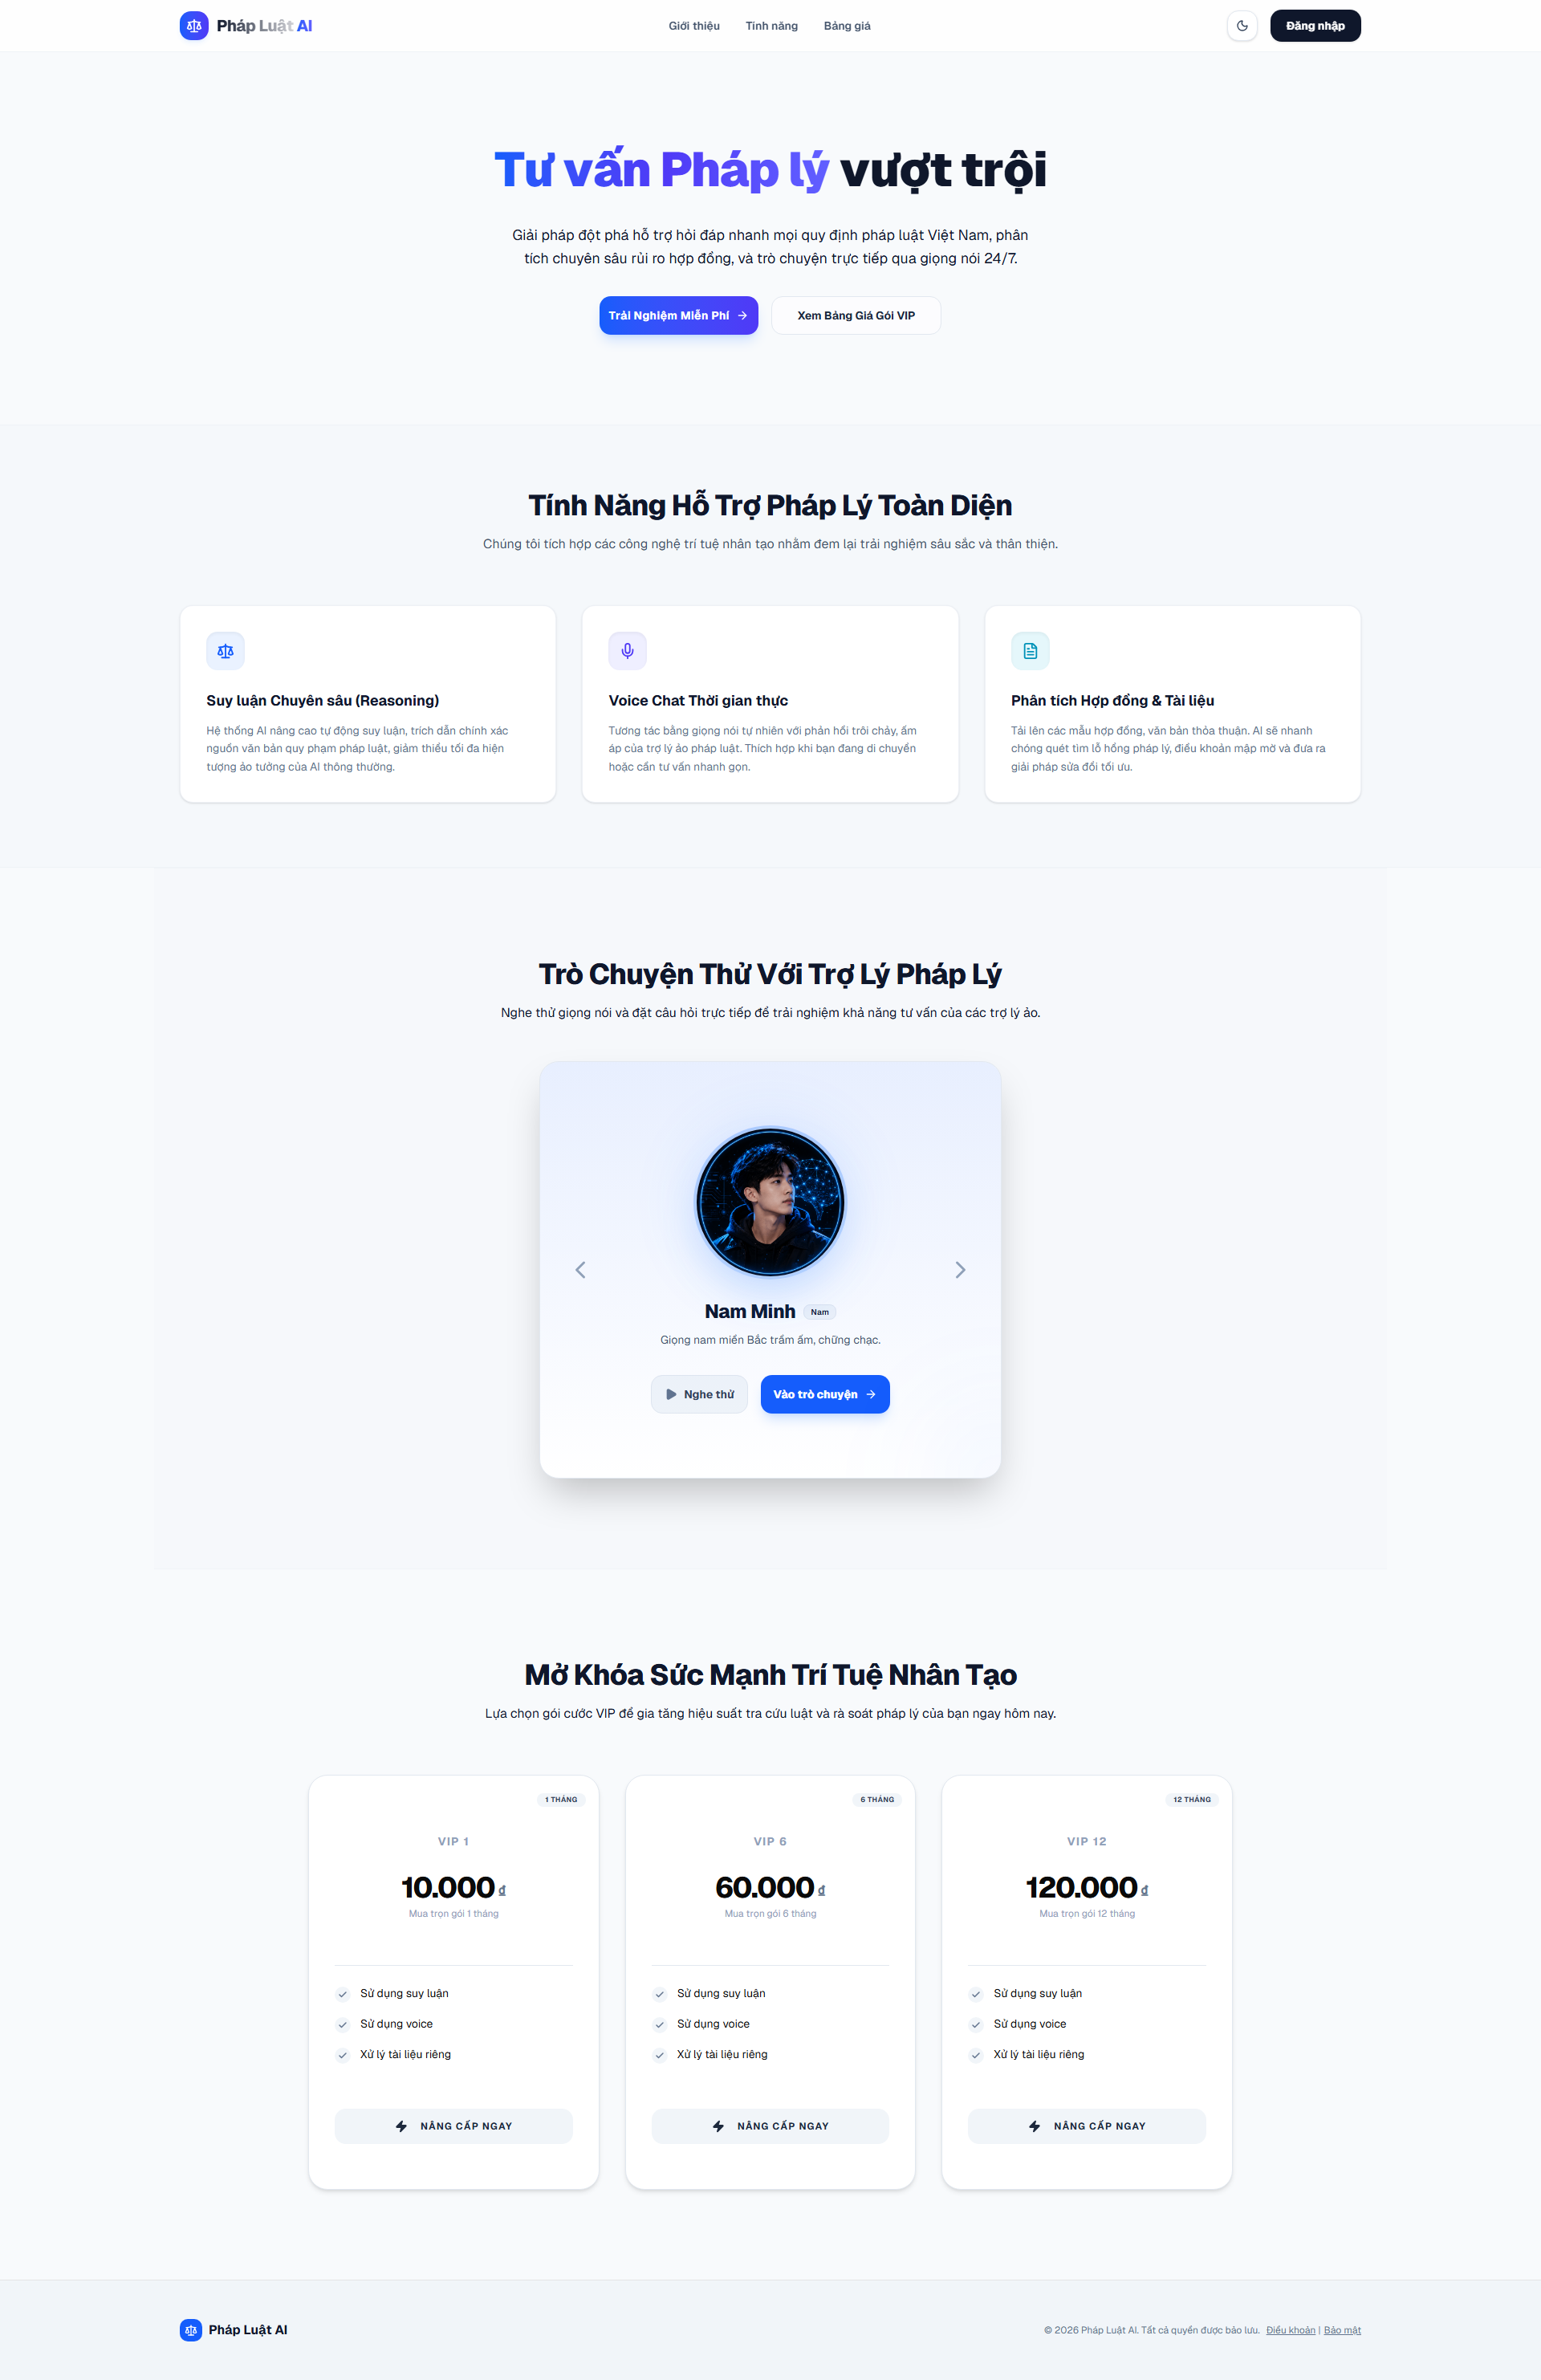
\includegraphics[width=0.92\textwidth]{pictures/WebUI/WebUI-GuestHome.png}
\caption{Giao diện trang chủ khách}
\end{figure}

\begin{enumerate}
\item Người dùng truy cập trang chủ.
\item Xem phần giới thiệu, gói VIP và danh sách nhân vật.
\item Chọn đăng nhập hoặc đăng ký để bắt đầu sử dụng hệ thống.
\end{enumerate}

\paragraph{Đăng ký tài khoản}

\begin{figure}[H]
\centering
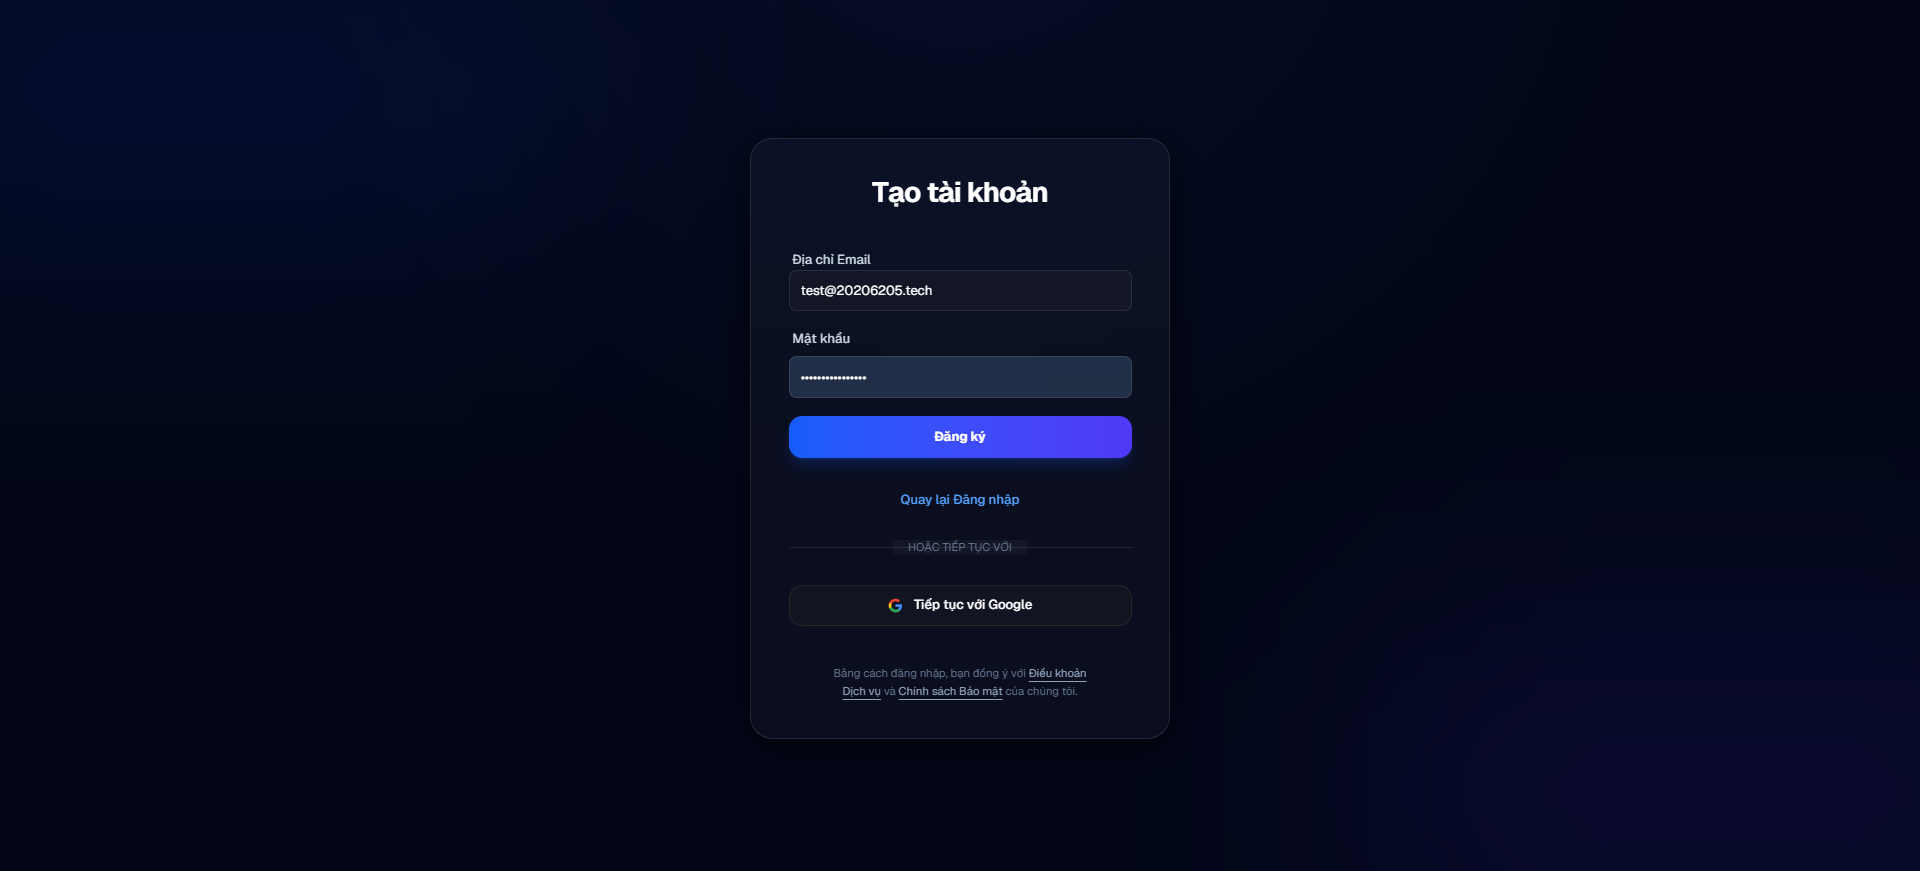
\includegraphics[width=0.5\textwidth]{pictures/WebUI/WebUI-GuestRegister.png}
\caption{Giao diện đăng ký tài khoản}
\end{figure}

\begin{enumerate}
\item Nhập email và mật khẩu.
\item Bấm nút đăng ký.
\item Kiểm tra thông báo yêu cầu xác thực email.
\end{enumerate}

\paragraph{Thông báo xác thực email}

\begin{figure}[H]
\centering
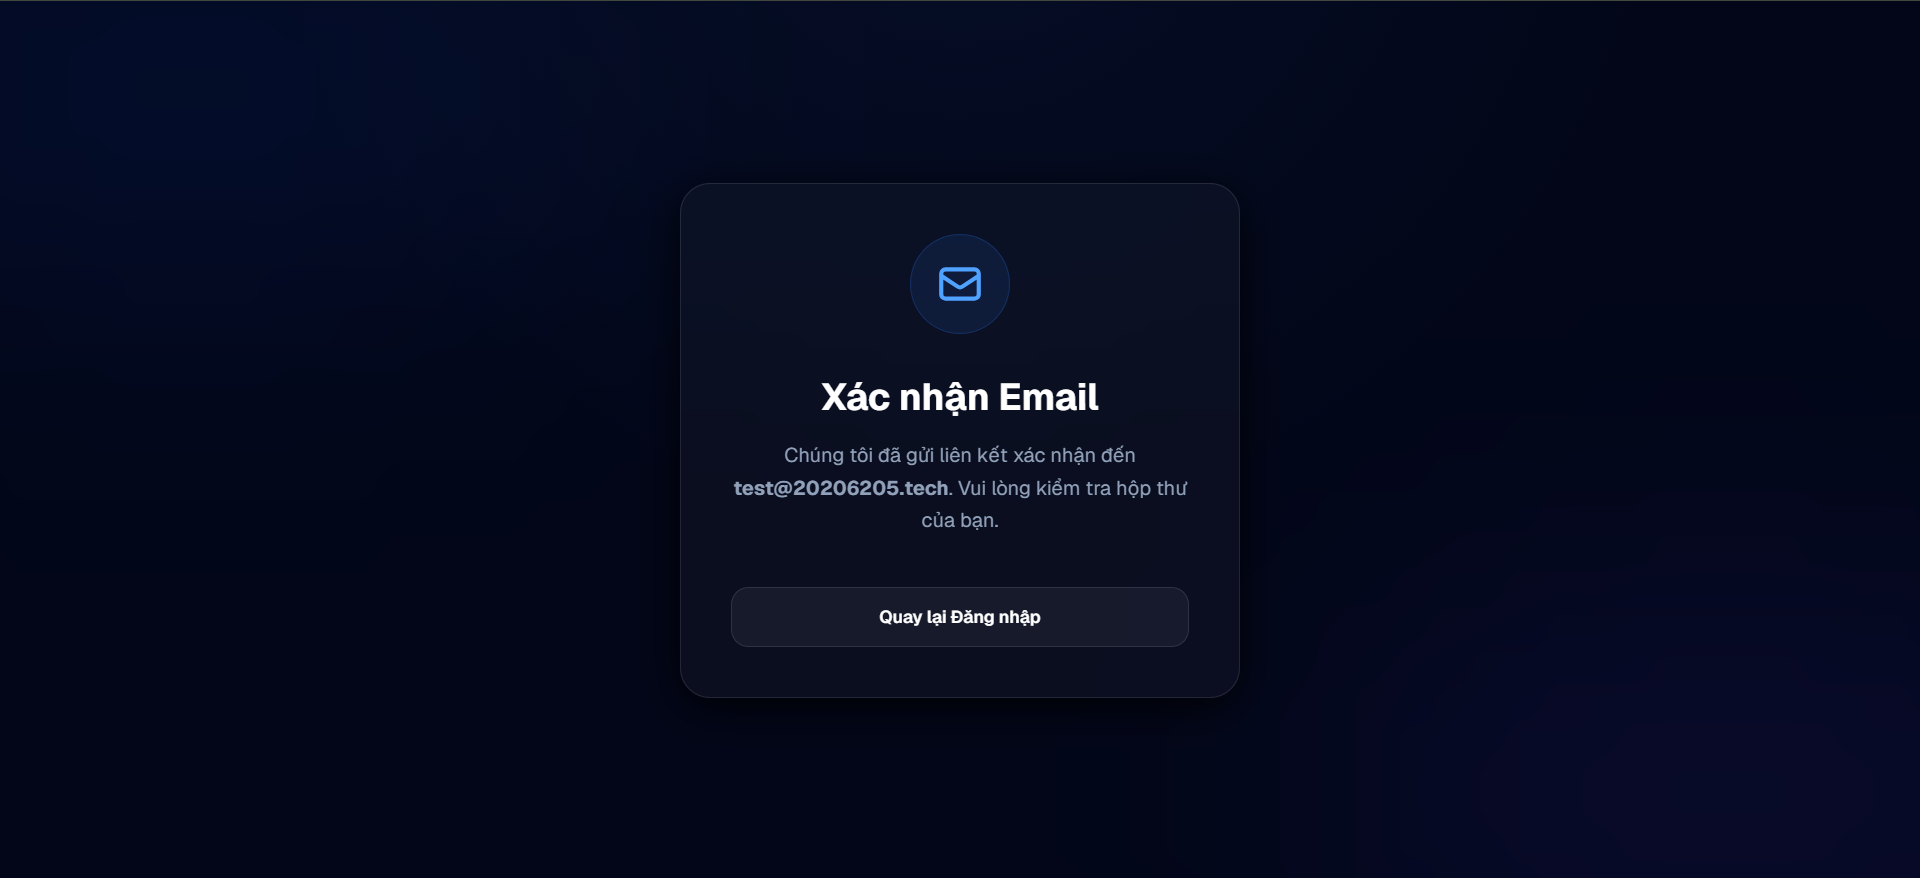
\includegraphics[width=0.5\textwidth]{pictures/WebUI/WebUI-GuestSignupConfirmEmail.png}
\caption{Giao diện thông báo xác thực email}
\end{figure}

\begin{enumerate}
\item Sau khi đăng ký, hệ thống hiển thị trạng thái chờ xác thực.
\item Người dùng mở hộp thư email đã đăng ký.
\item Bấm liên kết xác thực để kích hoạt tài khoản.
\end{enumerate}

\paragraph{Email xác thực đăng ký}

\begin{figure}[H]
\centering
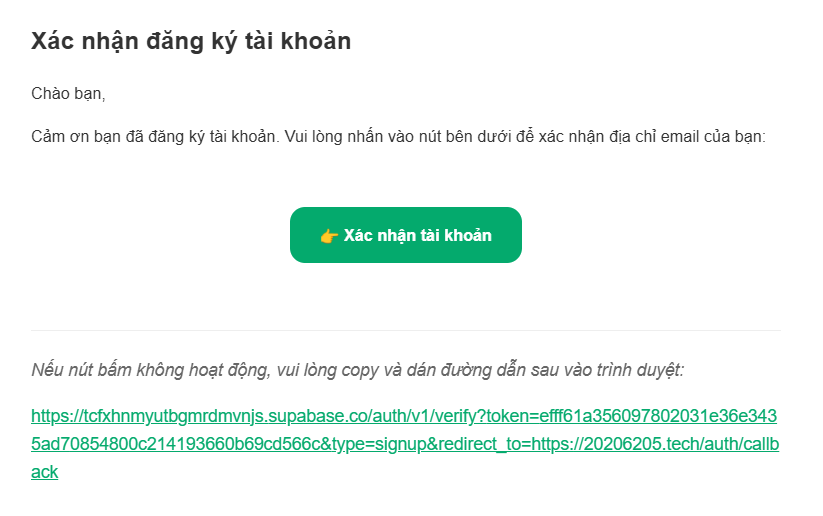
\includegraphics[width=0.5\textwidth]{pictures/WebUI/WebUI-GuestRegistrationEmail.png}
\caption{Giao diện email xác thực đăng ký}
\end{figure}

\begin{enumerate}
\item Mở email xác thực từ hệ thống.
\item Kiểm tra đúng địa chỉ email và nội dung xác thực.
\item Bấm liên kết xác nhận để quay lại hệ thống.
\end{enumerate}

\paragraph{Đăng nhập}

\begin{figure}[H]
\centering
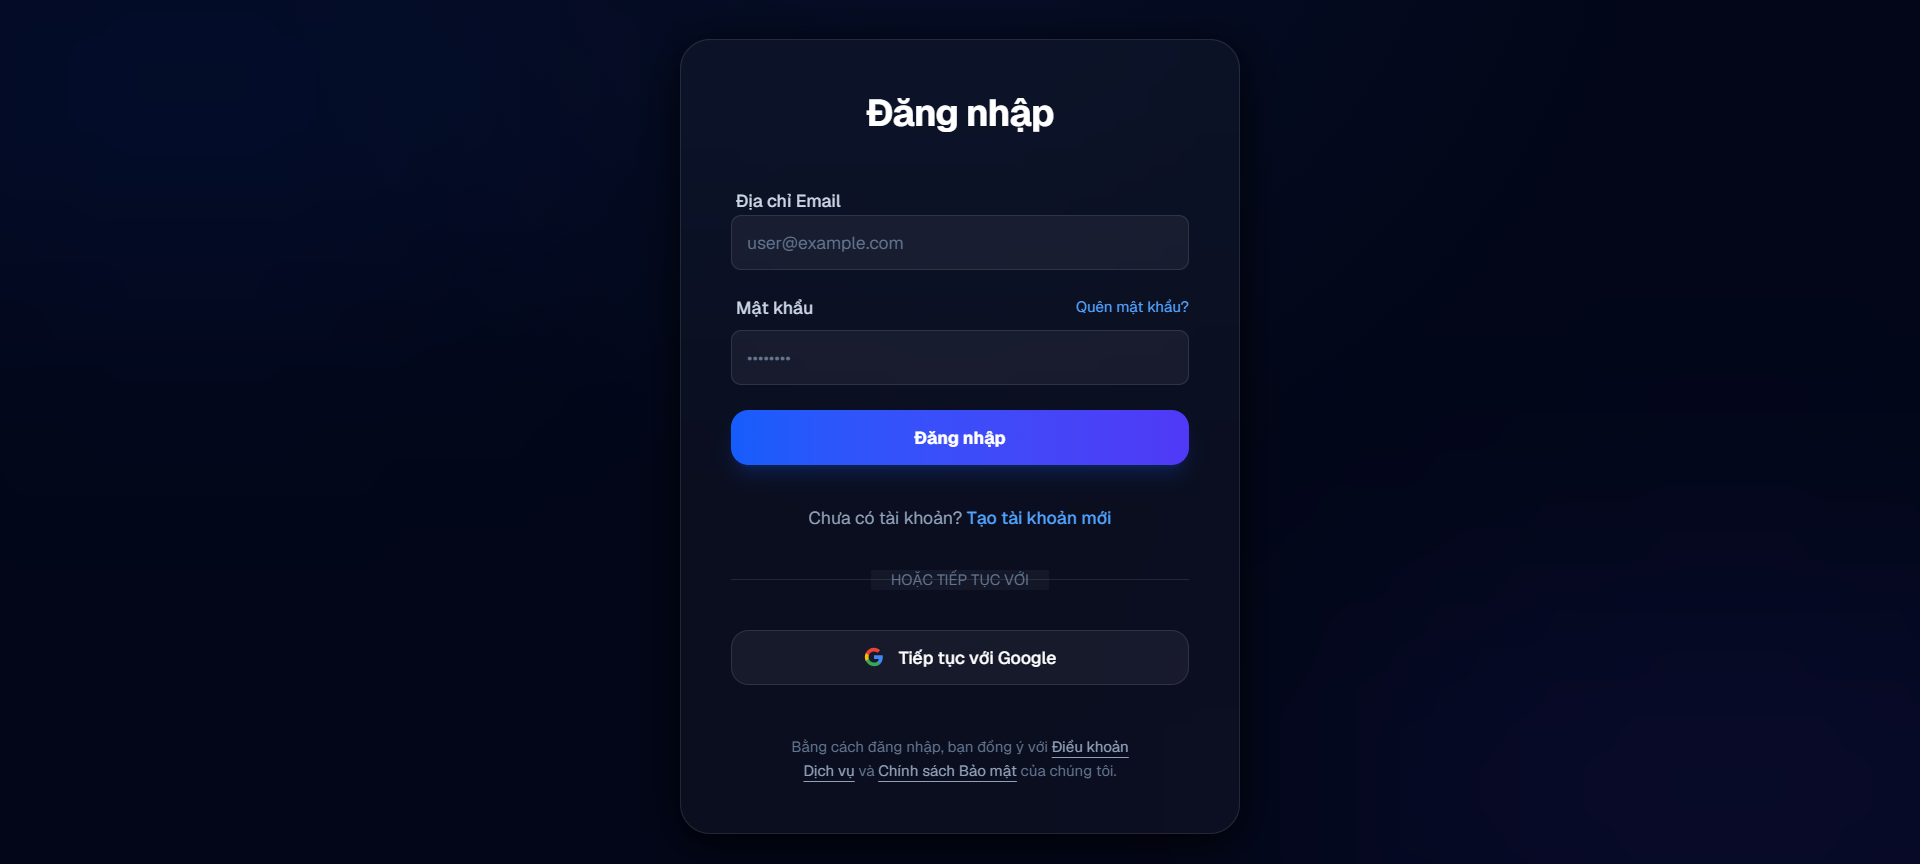
\includegraphics[width=0.65\textwidth]{pictures/WebUI/WebUI-GuestLogin.png}
\caption{Giao diện đăng nhập}
\end{figure}

\begin{enumerate}
\item Nhập email và mật khẩu.
\item Bấm đăng nhập.
\item Do bắt buộc bật MFA, hệ thống chuyển sang bước xác thực bổ sung.
\end{enumerate}

\paragraph{Thiết lập MFA bằng mã QR}

\begin{figure}[H]
\centering
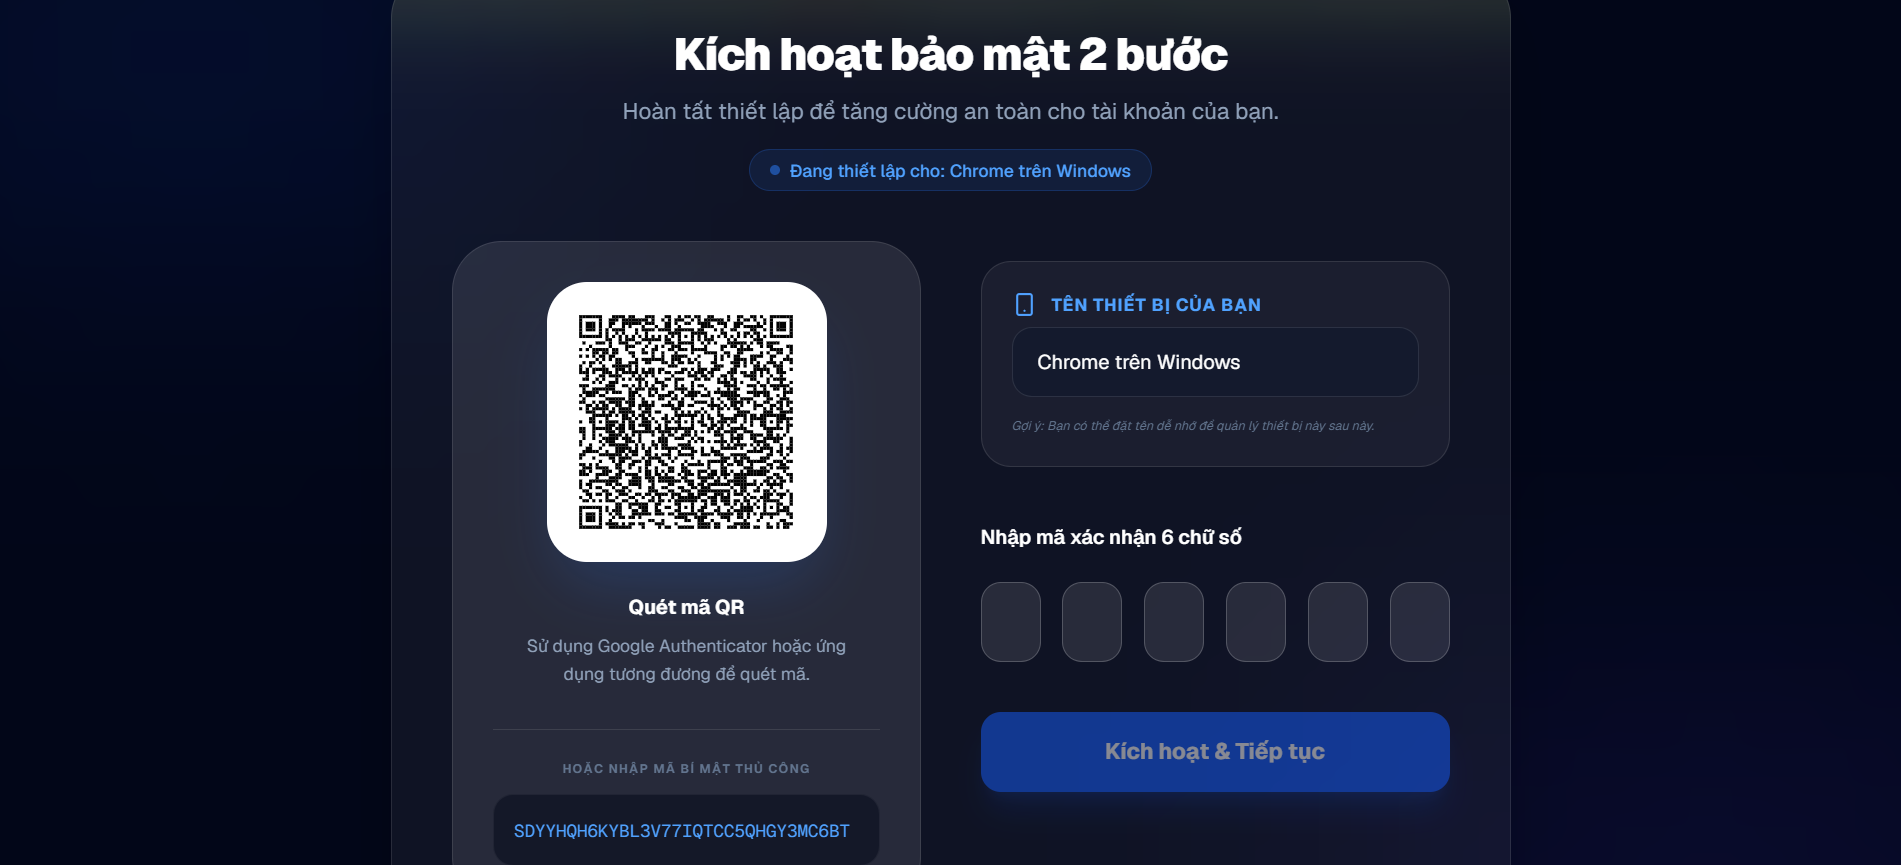
\includegraphics[width=0.65\textwidth]{pictures/WebUI/WebUI-MfaQrSetup.png}
\caption{Giao diện thiết lập MFA bằng mã QR}
\end{figure}

\begin{enumerate}
\item Mở ứng dụng xác thực trên điện thoại.
\item Quét mã QR hiển thị trên màn hình.
\item Lưu cấu hình MFA trong ứng dụng xác thực.
\end{enumerate}

\paragraph{Xác minh mã MFA}

\begin{figure}[H]
\centering
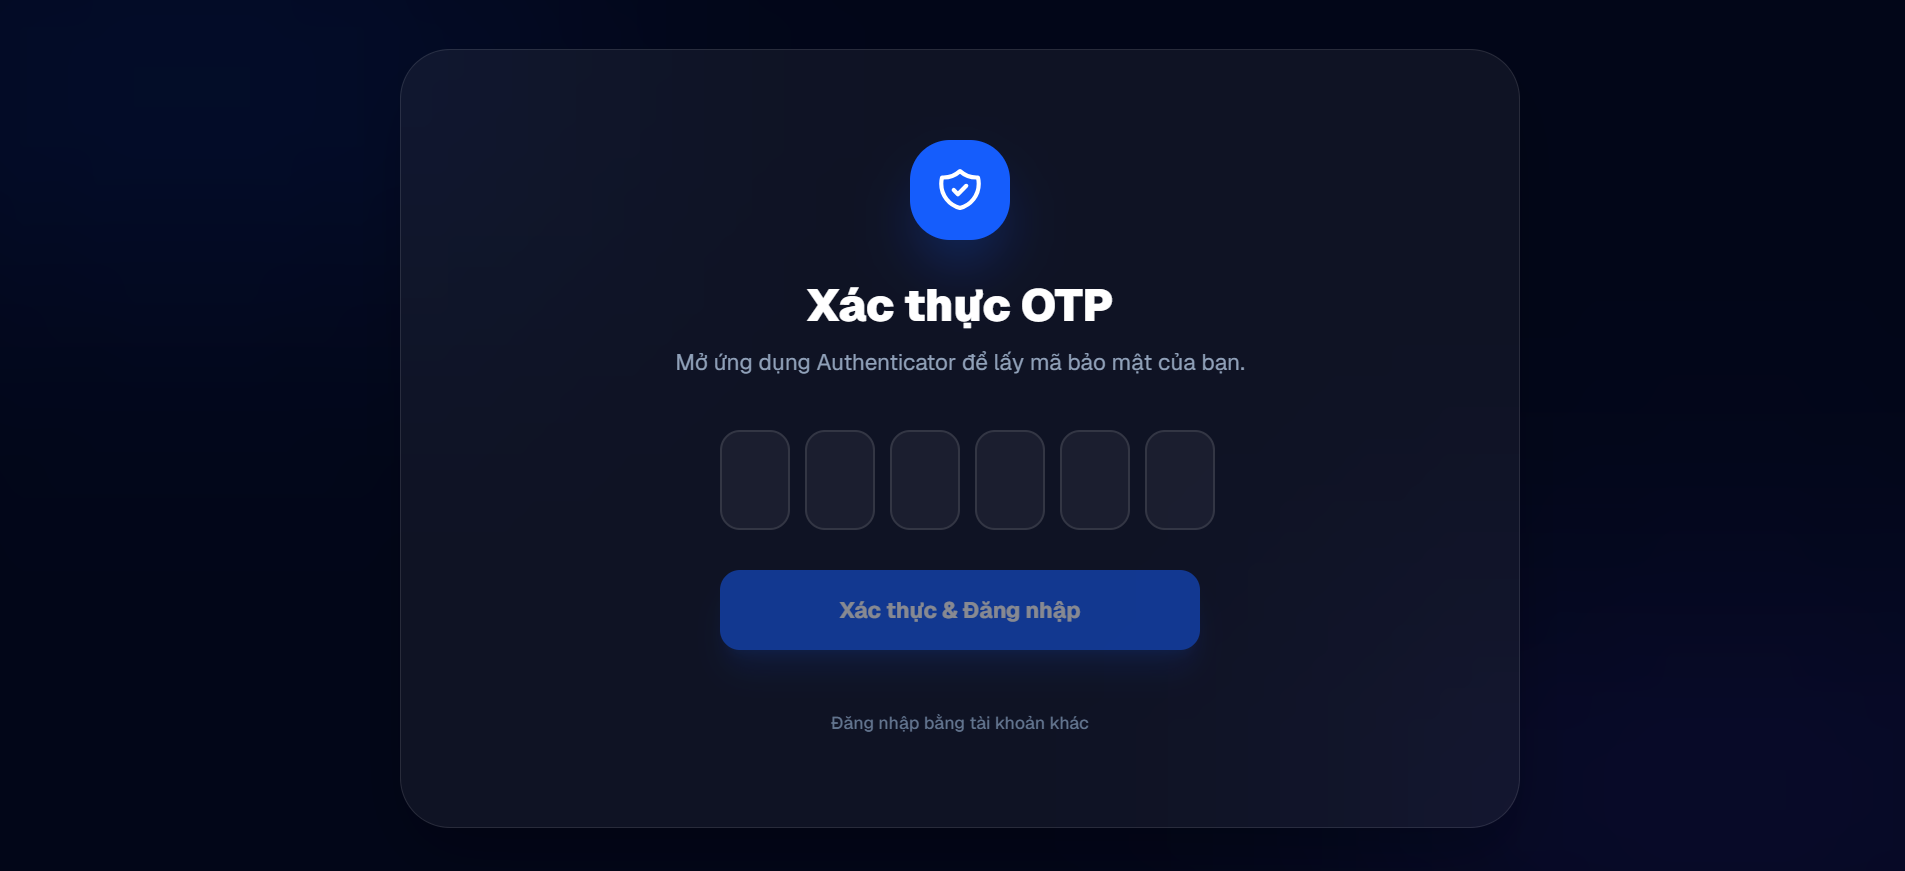
\includegraphics[width=0.65\textwidth]{pictures/WebUI/WebUI-MfaCodeVerify.png}
\caption{Giao diện xác minh mã MFA}
\end{figure}

\begin{enumerate}
\item Lấy mã TOTP mới nhất từ ứng dụng xác thực.
\item Nhập mã TOTP vào màn hình xác minh.
\item Bấm xác nhận để hoàn tất đăng nhập hoặc kích hoạt MFA.
\end{enumerate}

\paragraph{Hồ sơ người dùng}

\begin{figure}[H]
\centering
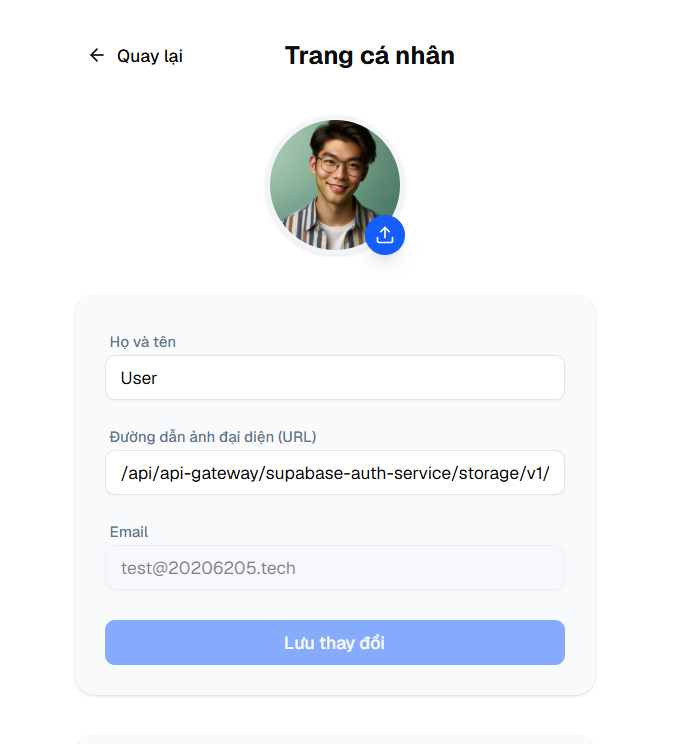
\includegraphics[width=0.6\textwidth]{pictures/WebUI/WebUI-UserProfile.png}
\caption{Giao diện hồ sơ người dùng}
\end{figure}

\begin{enumerate}
\item Mở trang hồ sơ cá nhân.
\item Xem hoặc cập nhật thông tin hiển thị.
\item Lưu thay đổi để hệ thống cập nhật hồ sơ.
\end{enumerate}

\paragraph{Đổi mật khẩu và MFA}

\begin{figure}[H]
\centering
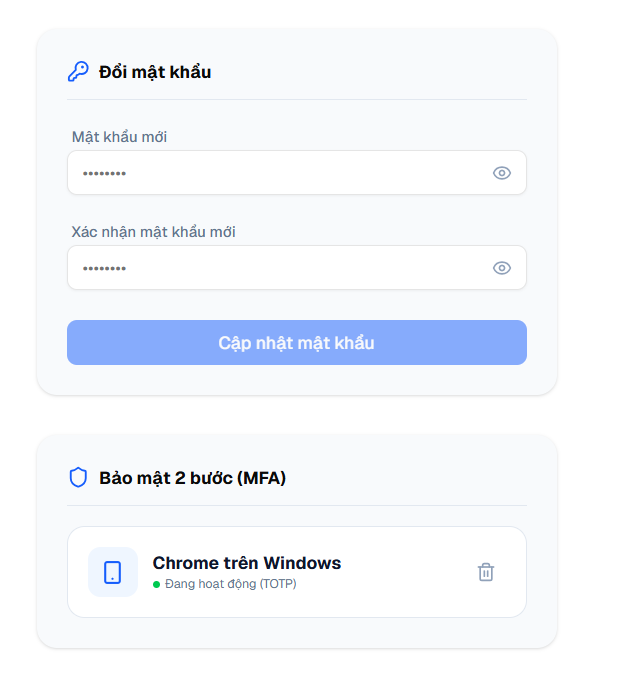
\includegraphics[width=0.6\textwidth]{pictures/WebUI/WebUI-ChangePasswordAndMfa.png}
\caption{Giao diện đổi mật khẩu và MFA}
\end{figure}

\begin{enumerate}
\item Mở phần bảo mật tài khoản.
\item Đổi mật khẩu hoặc quản lý xác thực MFA.
\item Xác nhận thao tác theo yêu cầu của hệ thống.
\end{enumerate}

\paragraph{Cài đặt người dùng}

\begin{figure}[H]
\centering
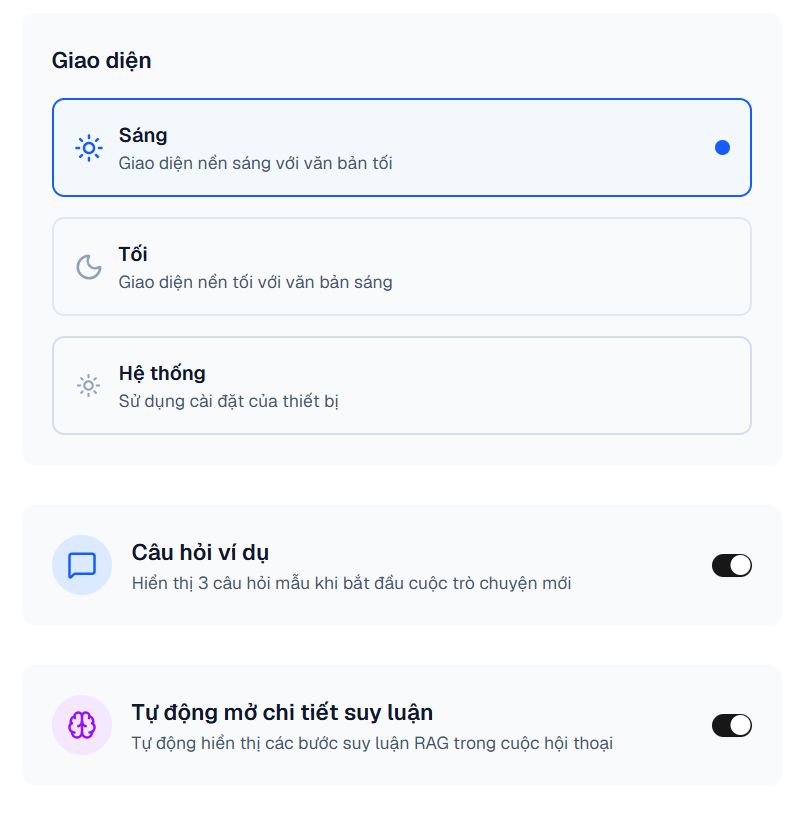
\includegraphics[width=0.7\textwidth]{pictures/WebUI/WebUI-UserSettings.png}
\caption{Giao diện cài đặt người dùng}
\end{figure}

\begin{enumerate}
\item Mở trang cài đặt.
\item Điều chỉnh các tùy chọn cá nhân như giao diện, giọng nói hoặc cấu hình trò chuyện.
\item Bấm lưu để áp dụng cấu hình.
\end{enumerate}

\paragraph{Khôi phục mật khẩu}

\begin{figure}[H]
\centering
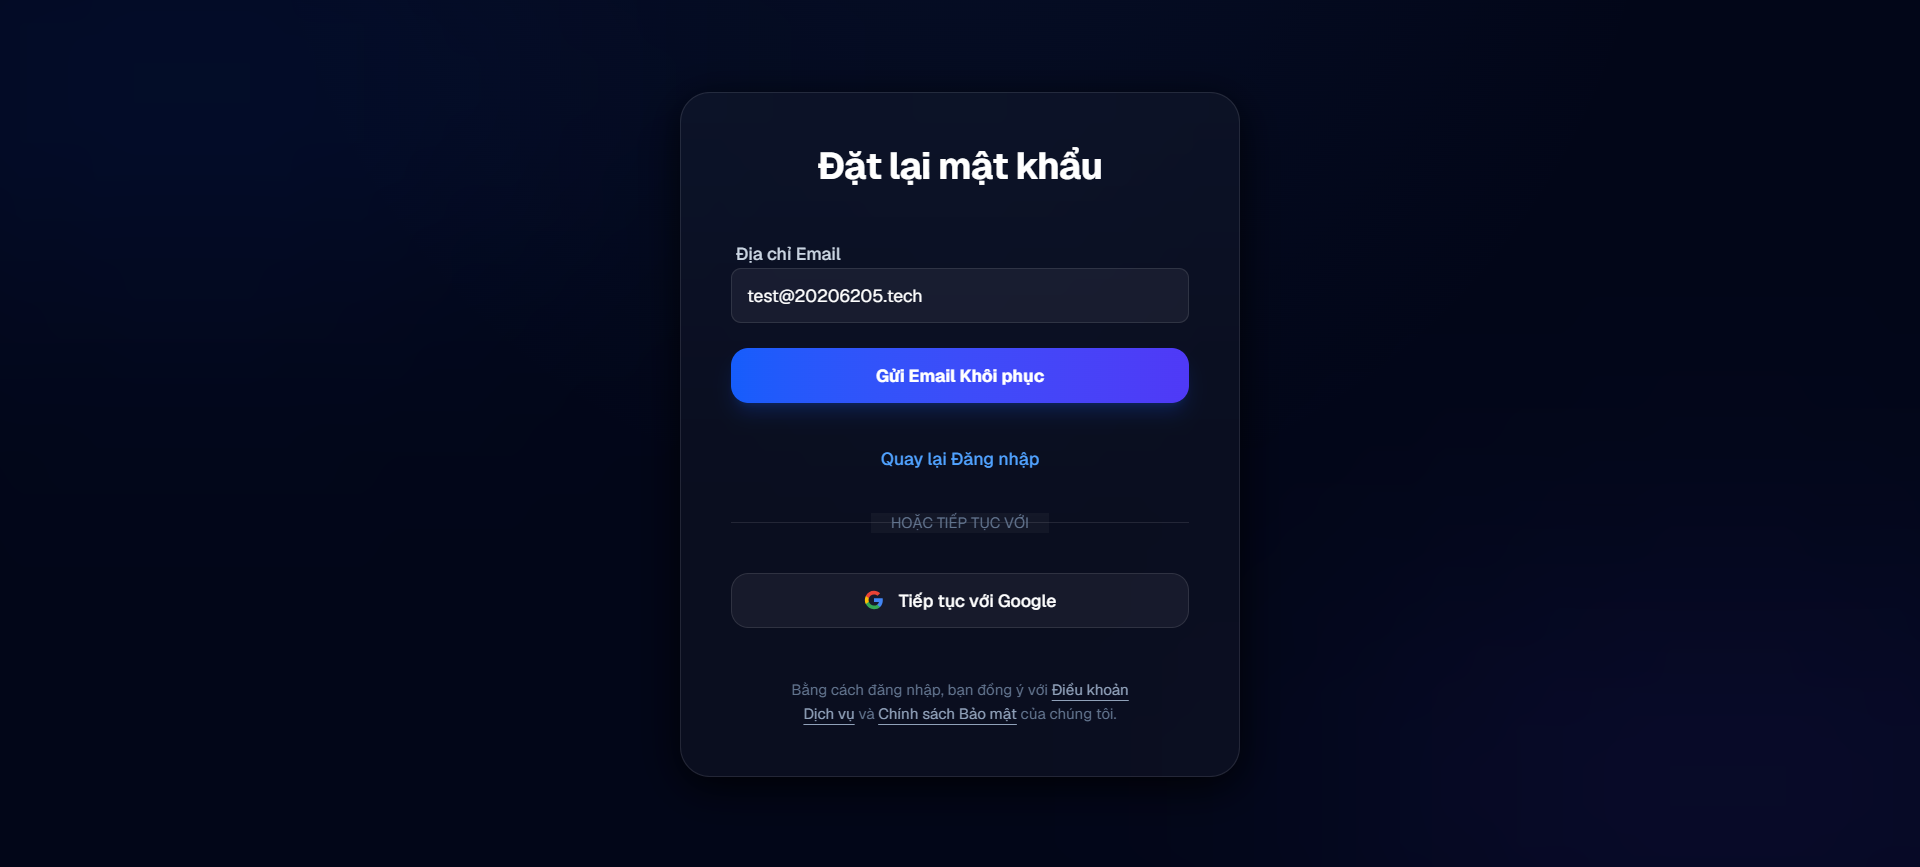
\includegraphics[width=0.6\textwidth]{pictures/WebUI/WebUI-ResetPassword.png}
\caption{Giao diện khôi phục mật khẩu}
\end{figure}

\begin{enumerate}
\item Nhập email đã đăng ký.
\item Bấm gửi yêu cầu khôi phục.
\item Mở email khôi phục mật khẩu và làm theo hướng dẫn.
\end{enumerate}

\paragraph{Email khôi phục mật khẩu}

\begin{figure}[H]
\centering
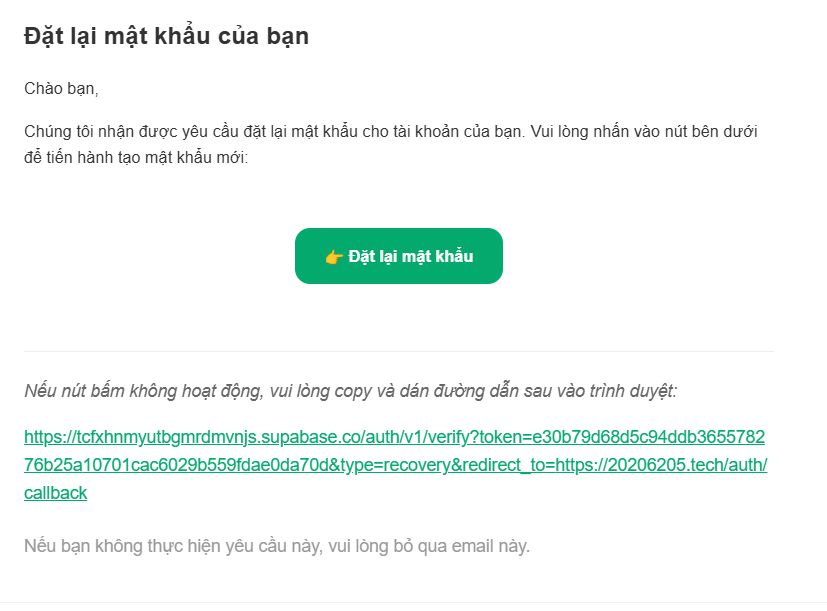
\includegraphics[width=0.92\textwidth]{pictures/WebUI/WebUI-PasswordResetEmail.png}
\caption{Giao diện email khôi phục mật khẩu}
\end{figure}

\begin{enumerate}
\item Mở email khôi phục mật khẩu.
\item Bấm liên kết đặt lại mật khẩu.
\item Nhập mật khẩu mới trên màn hình được chuyển hướng.
\end{enumerate}

% \subsubsection{Trò chuyện, ghi chú và chia sẻ}

\paragraph{Trò chuyện văn bản}

\begin{figure}[H]
\centering
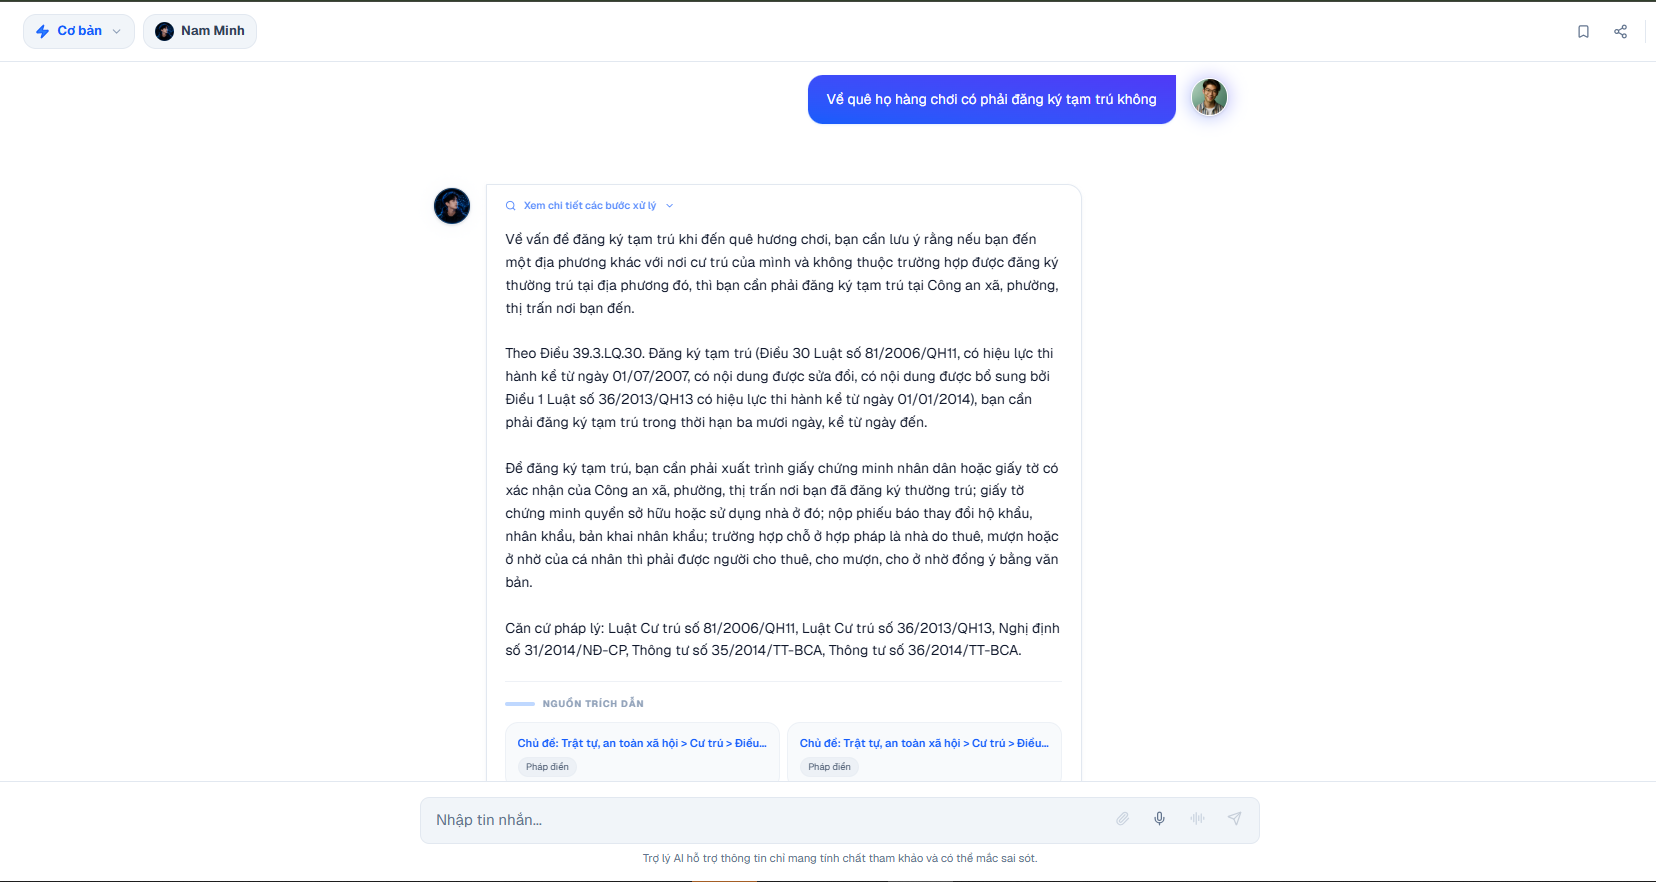
\includegraphics[width=0.92\textwidth]{pictures/WebUI/WebUI-ChatText.png}
\caption{Giao diện trò chuyện văn bản}
\end{figure}

\begin{enumerate}
\item Nhập câu hỏi vào khung trò chuyện.
\item Chọn tùy chọn bổ sung nếu cần, ví dụ suy luận hoặc tài liệu đính kèm.
\item Gửi câu hỏi và theo dõi phản hồi dạng streaming.
\end{enumerate}

\paragraph{Trò chuyện bằng micro}

\begin{figure}[H]
\centering
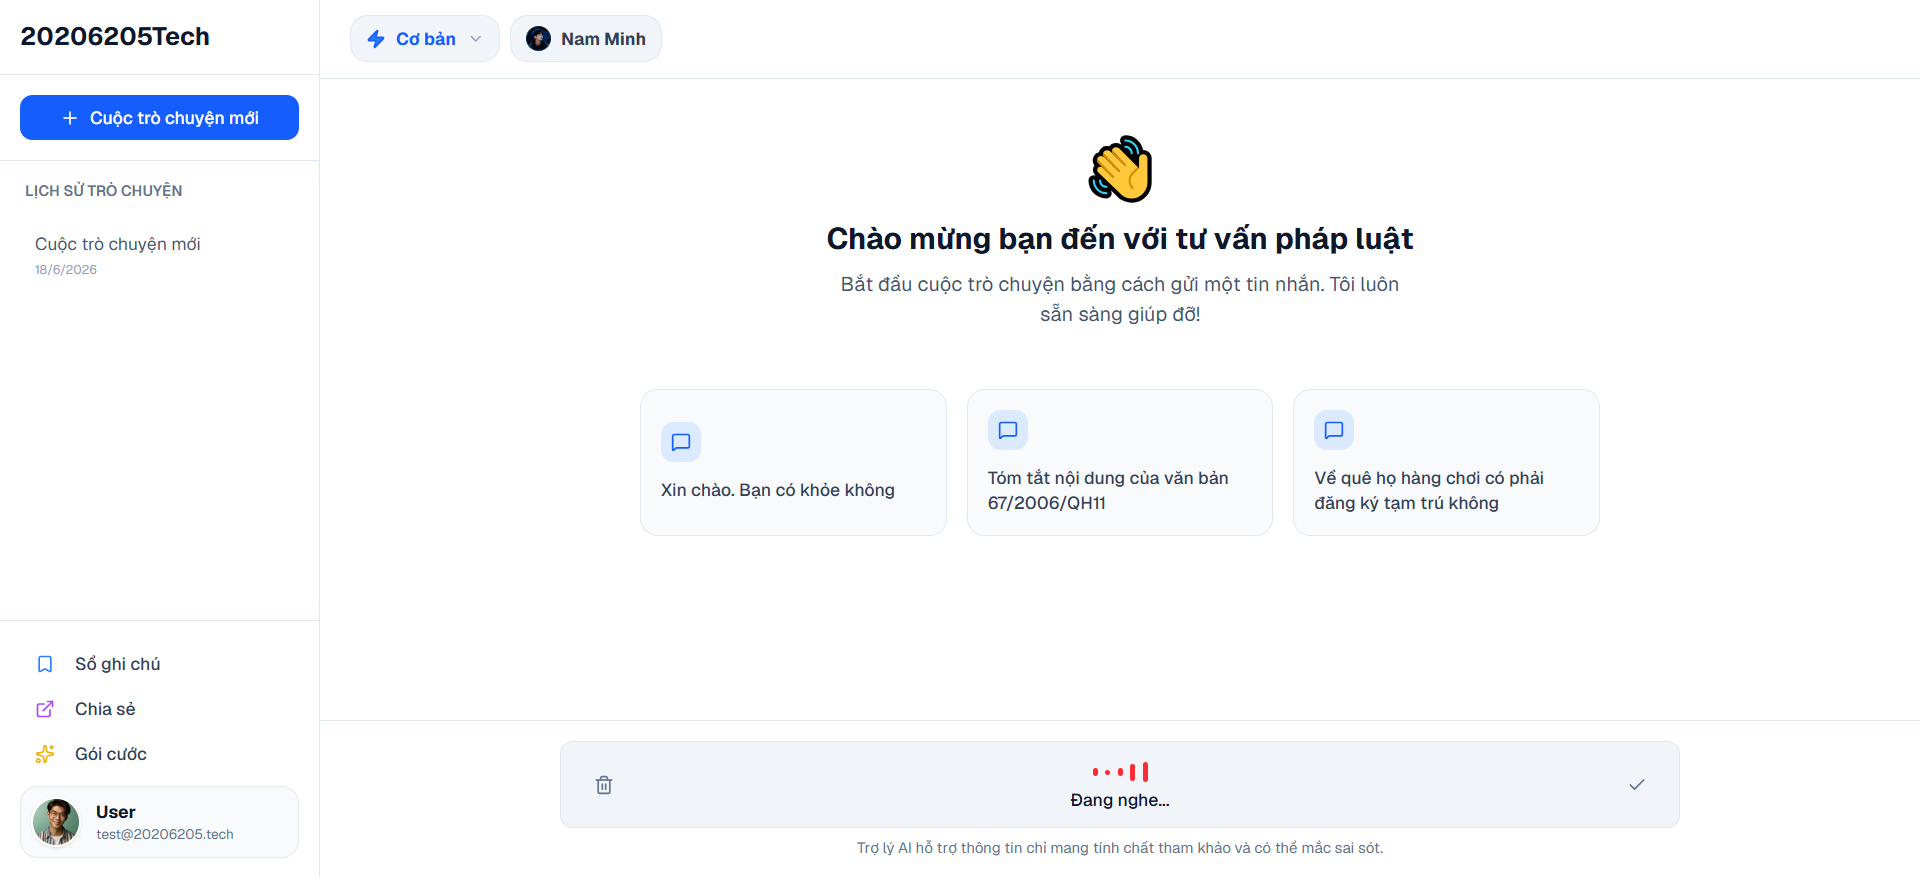
\includegraphics[width=0.7\textwidth]{pictures/WebUI/WebUI-ChatMicrophone.png}
\caption{Giao diện trò chuyện bằng micro}
\end{figure}

\begin{enumerate}
\item Bấm biểu tượng micro để bắt đầu nhập bằng giọng nói.
\item Cho phép trình duyệt truy cập micro nếu được hỏi.
\item Nói câu hỏi và chờ hệ thống xử lý.
\end{enumerate}

\paragraph{Tạo ghi chú đánh dấu}

\begin{figure}[H]
\centering
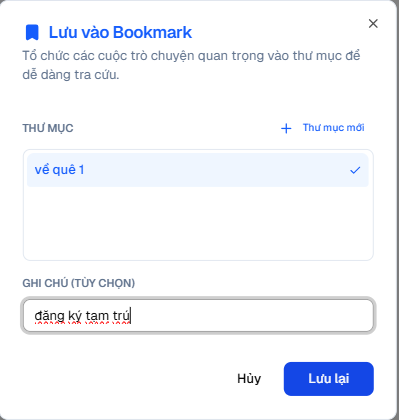
\includegraphics[width=0.7\textwidth]{pictures/WebUI/WebUI-BookmarkNoteCreate.png}
\caption{Giao diện tạo ghi chú đánh dấu}
\end{figure}

\begin{enumerate}
\item Chọn cuộc trò chuyện cần lưu.
\item Chọn hoặc tạo thư mục đánh dấu.
\item Nhập ghi chú và bấm lưu.
\end{enumerate}

\paragraph{Quản lý ghi chú đánh dấu}

\begin{figure}[H]
\centering
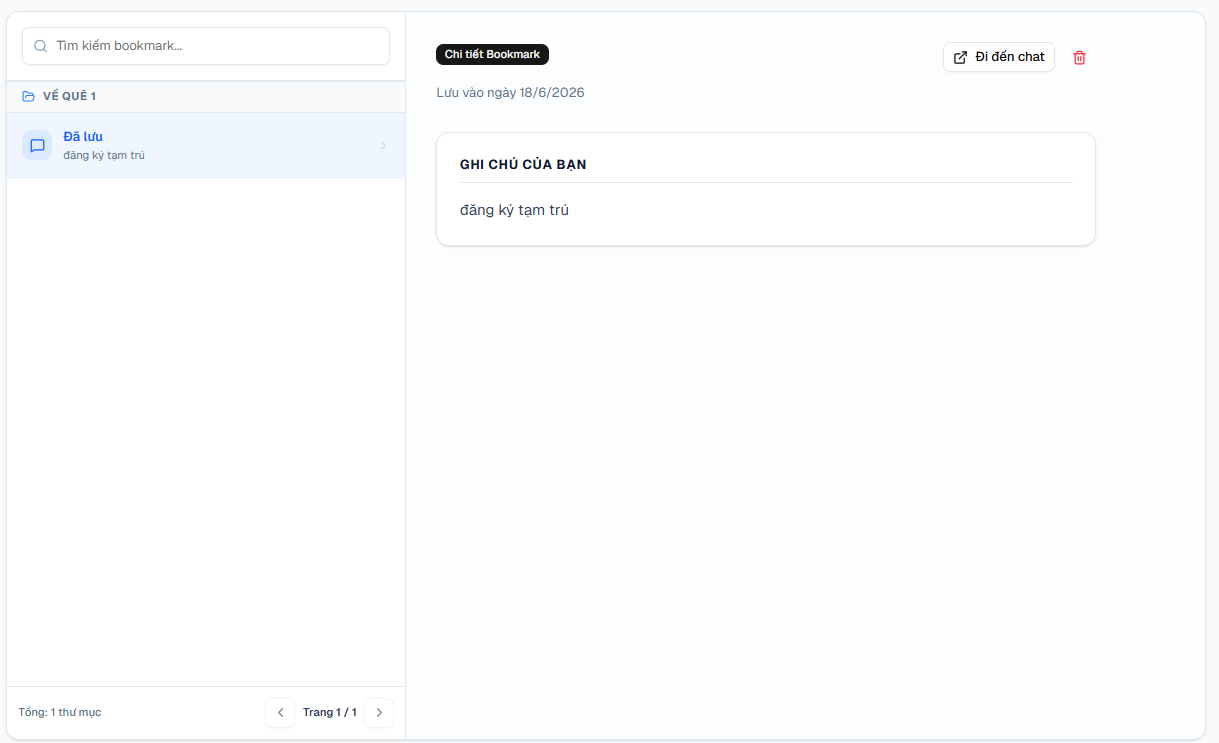
\includegraphics[width=0.7\textwidth]{pictures/WebUI/WebUI-BookmarkNoteManage.png}
\caption{Giao diện quản lý ghi chú đánh dấu}
\end{figure}

\begin{enumerate}
\item Mở danh sách đánh dấu.
\item Tìm cuộc trò chuyện hoặc thư mục cần quản lý.
\item Chỉnh sửa ghi chú, đổi thư mục hoặc mở cuộc trò chuyện.
\end{enumerate}

\paragraph{Tạo liên kết chia sẻ}

\begin{figure}[H]
\centering
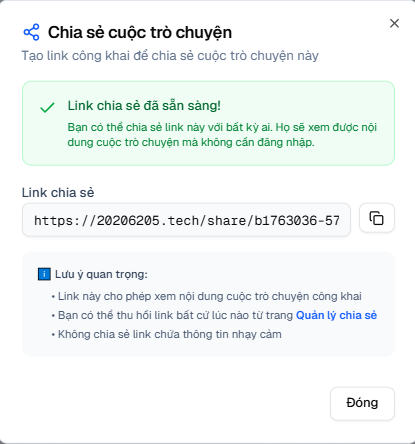
\includegraphics[width=0.7\textwidth]{pictures/WebUI/WebUI-ShareCreate.png}
\caption{Giao diện tạo liên kết chia sẻ}
\end{figure}

\begin{enumerate}
\item Mở cuộc trò chuyện cần chia sẻ.
\item Bấm tạo liên kết chia sẻ.
\item Sao chép liên kết sau khi hệ thống tạo xong.
\end{enumerate}

\paragraph{Quản lý chia sẻ}

\begin{figure}[H]
\centering
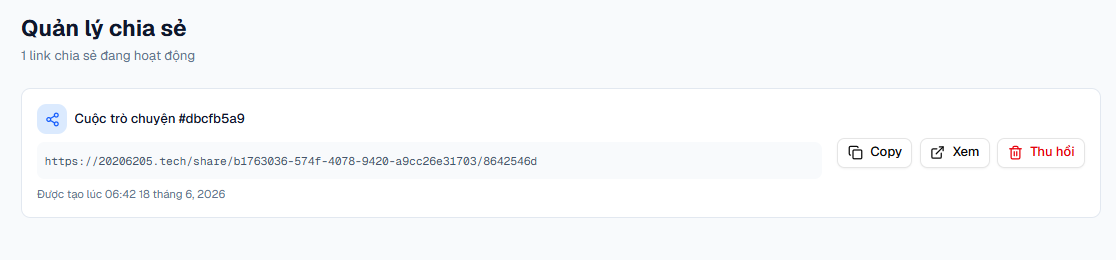
\includegraphics[width=0.92\textwidth]{pictures/WebUI/WebUI-ShareManage.png}
\caption{Giao diện quản lý chia sẻ}
\end{figure}

\begin{enumerate}
\item Mở danh sách liên kết chia sẻ.
\item Kiểm tra trạng thái từng liên kết.
\item Thu hồi liên kết nếu không muốn tiếp tục chia sẻ.
\end{enumerate}

\paragraph{Liên kết chia sẻ không khả dụng}

\begin{figure}[H]
\centering
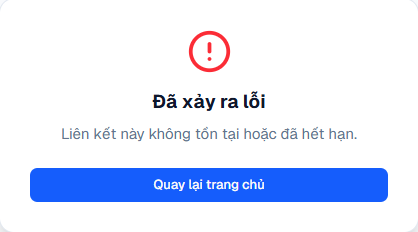
\includegraphics[width=0.5\textwidth]{pictures/WebUI/WebUI-ShareLinkUnavailable.png}
\caption{Giao diện liên kết chia sẻ không khả dụng}
\end{figure}

\begin{enumerate}
\item Người nhận mở liên kết chia sẻ.
\item Nếu liên kết đã bị thu hồi hoặc không tồn tại, hệ thống hiển thị thông báo liên kết không tồn tại hoặc đã hết hạn.
\item Liên hệ người chia sẻ để nhận liên kết mới nếu cần.
\end{enumerate}

\paragraph{Liên kết chia sẻ khả dụng}

\begin{figure}[H]
\centering
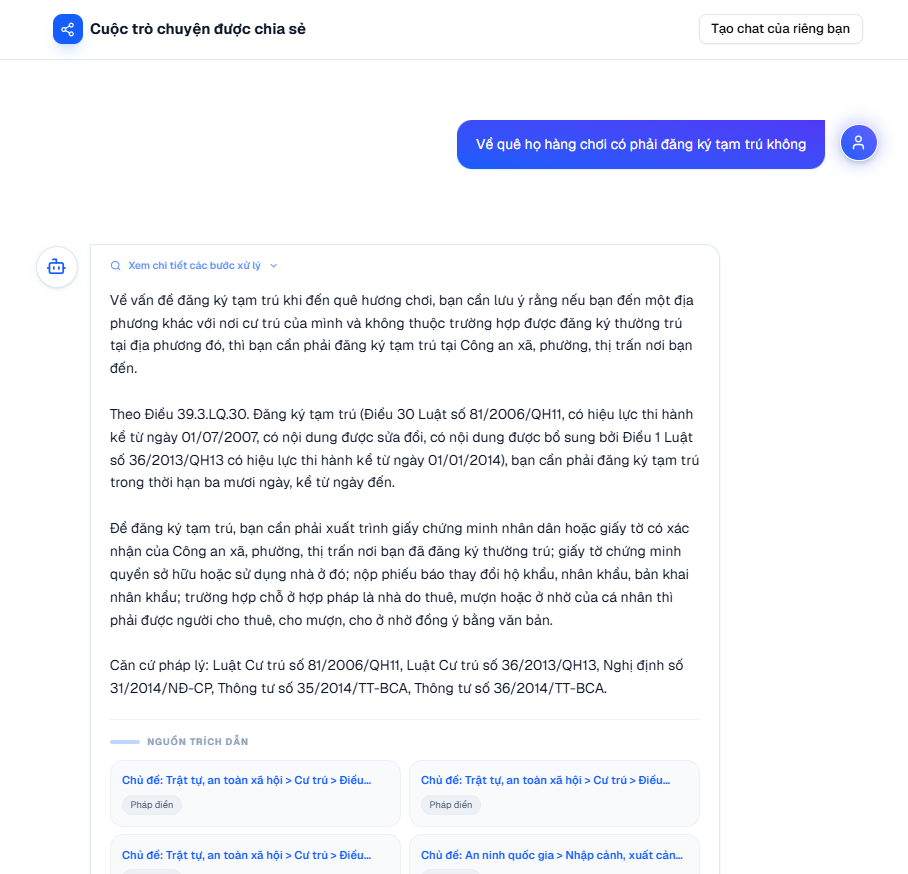
\includegraphics[width=0.55\textwidth]{pictures/WebUI/WebUI-ShareLinkDone.png}
\caption{Giao diện liên kết chia sẻ khả dụng}
\end{figure}

\begin{enumerate}
\item Mở liên kết chia sẻ hợp lệ.
\item Xem nội dung trò chuyện được chia sẻ.
\item Dùng nội dung này để tham khảo cuộc trò chuyện.
\end{enumerate}

\paragraph{Thu hồi chia sẻ}

\begin{figure}[H]
\centering
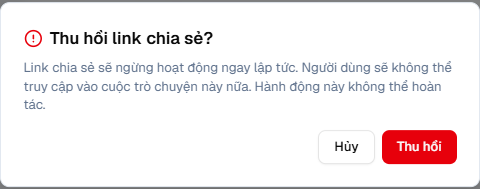
\includegraphics[width=0.7\textwidth]{pictures/WebUI/WebUI-ShareRevoke.png}
\caption{Giao diện thu hồi chia sẻ}
\end{figure}

\begin{enumerate}
\item Chọn liên kết chia sẻ cần thu hồi.
\item Bấm thu hồi hoặc hủy chia sẻ.
\item Xác nhận thao tác để liên kết không còn truy cập được.
\end{enumerate}

\paragraph{Xóa cuộc trò chuyện}

\begin{figure}[H]
\centering
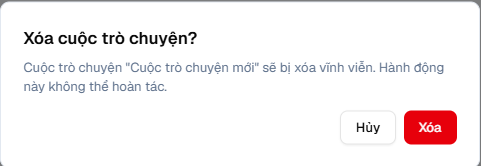
\includegraphics[width=0.7\textwidth]{pictures/WebUI/WebUI-ChatDelete.png}
\caption{Giao diện xóa cuộc trò chuyện}
\end{figure}

\begin{enumerate}
\item Chọn cuộc trò chuyện cần xóa.
\item Bấm thao tác xóa.
\item Xác nhận để hệ thống xóa hoặc ẩn cuộc trò chuyện khỏi danh sách.
\end{enumerate}

% \subsubsection{Quản trị hệ thống}

\paragraph{Quản lý gói VIP}

\begin{figure}[H]
\centering
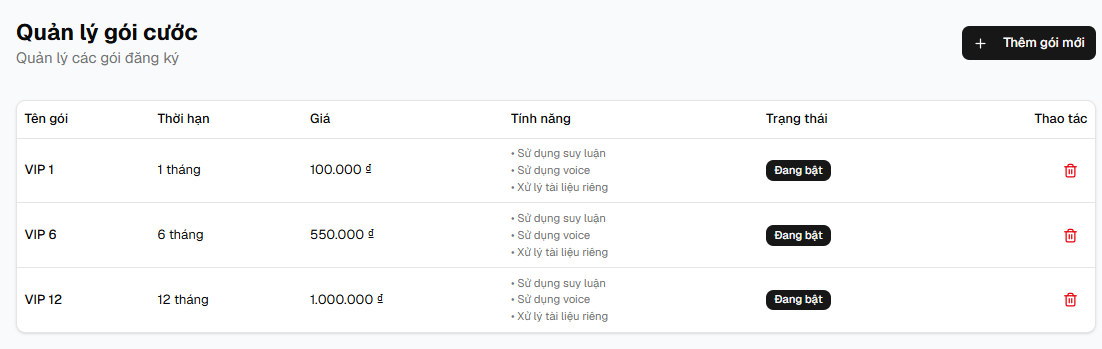
\includegraphics[width=0.92\textwidth]{pictures/WebUI/WebUI-AdminPlans.png}
\caption{Giao diện quản lý gói VIP}
\end{figure}

\begin{enumerate}
\item Quản trị viên mở trang quản lý gói VIP.
\item Xem danh sách gói hiện có.
\item Tạo mới, cập nhật hoặc vô hiệu hóa gói theo nhu cầu.
\end{enumerate}

\paragraph{Quản lý nhân vật}

\begin{figure}[H]
\centering
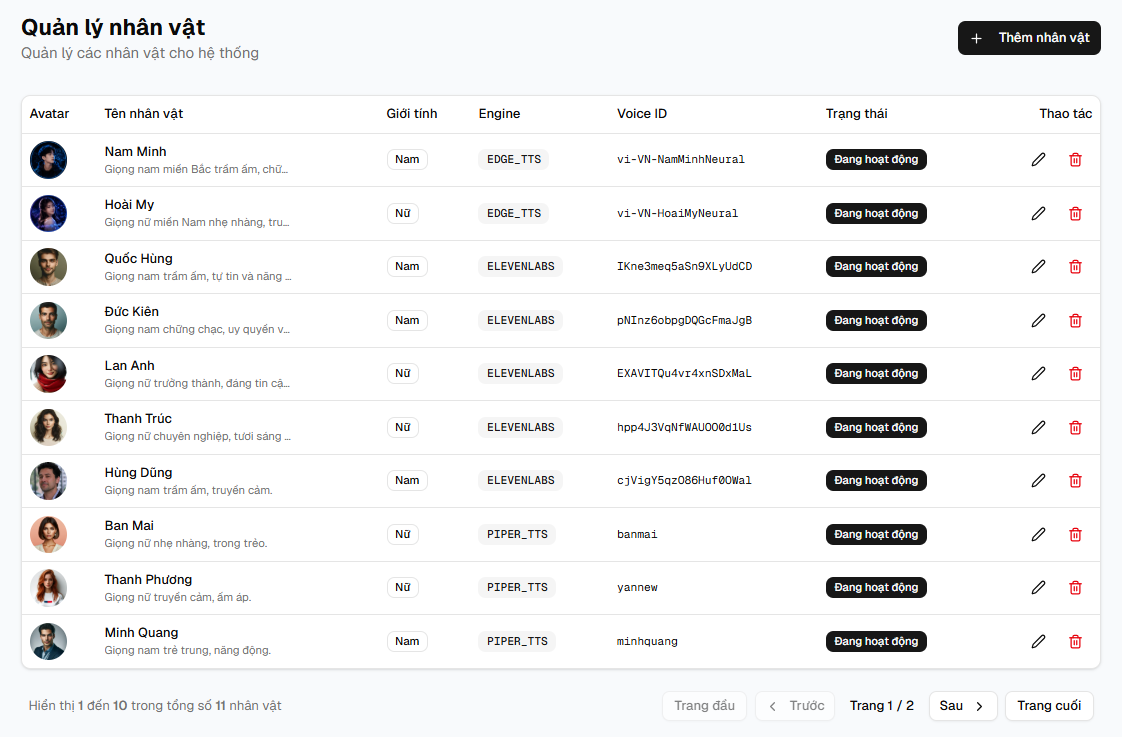
\includegraphics[width=0.92\textwidth]{pictures/WebUI/WebUI-AdminPersonas.png}
\caption{Giao diện quản lý nhân vật}
\end{figure}

\begin{enumerate}
\item Quản trị viên mở trang quản lý nhân vật.
\item Nhập thông tin nhân vật.
\item Lưu để nhân vật xuất hiện trong hệ thống.
\end{enumerate}

\paragraph{Quản lý công cụ dịch vụ giọng nói}

\begin{figure}[H]
\centering
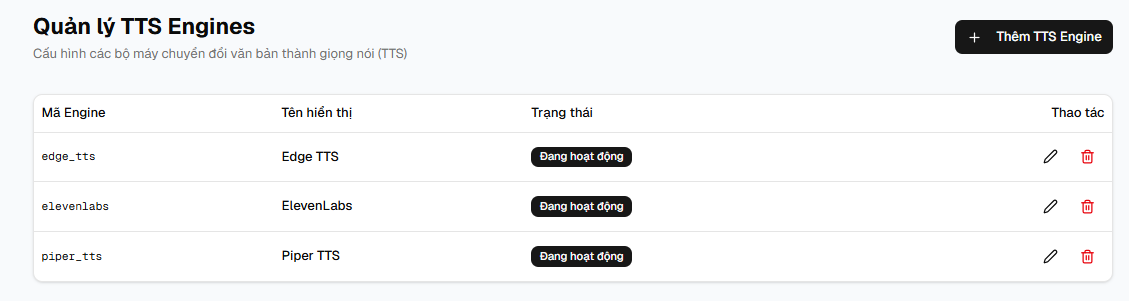
\includegraphics[width=0.99\textwidth]{pictures/WebUI/WebUI-AdminEngines.png}
\caption{Giao diện quản lý công cụ dịch vụ giọng nói}
\end{figure}

\begin{enumerate}
\item Quản trị viên mở trang cấu hình công cụ dịch vụ giọng nói.
\item Kiểm tra trạng thái các công cụ dịch vụ giọng nói đang hỗ trợ.
\item Bật, tắt hoặc cập nhật thông tin công cụ dịch vụ giọng nói.
\end{enumerate}

\paragraph{Quản lý giọng nói}

\begin{figure}[H]
\centering
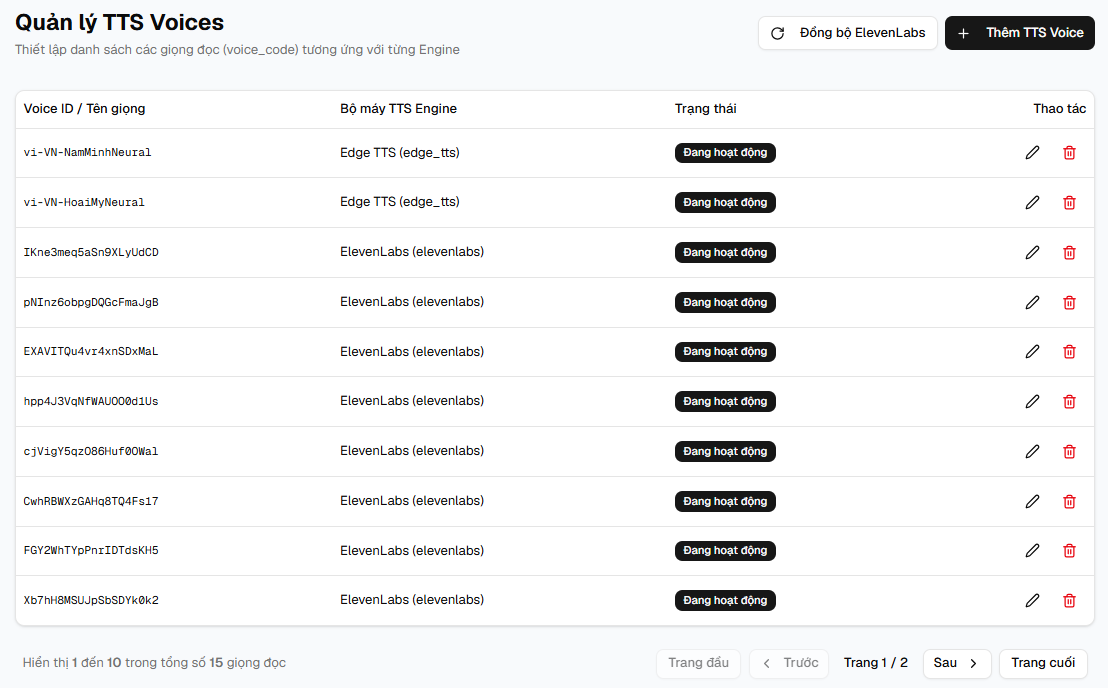
\includegraphics[width=0.92\textwidth]{pictures/WebUI/WebUI-AdminVoices.png}
\caption{Giao diện quản lý giọng nói}
\end{figure}

\begin{enumerate}
\item Quản trị viên mở trang giọng nói.
\item Đồng bộ hoặc cập nhật danh sách giọng nói.
\item Gắn giọng nói phù hợp cho nhân vật AI.
\end{enumerate}

\paragraph{Đường ống dữ liệu VBPL}

\begin{figure}[H]
\centering
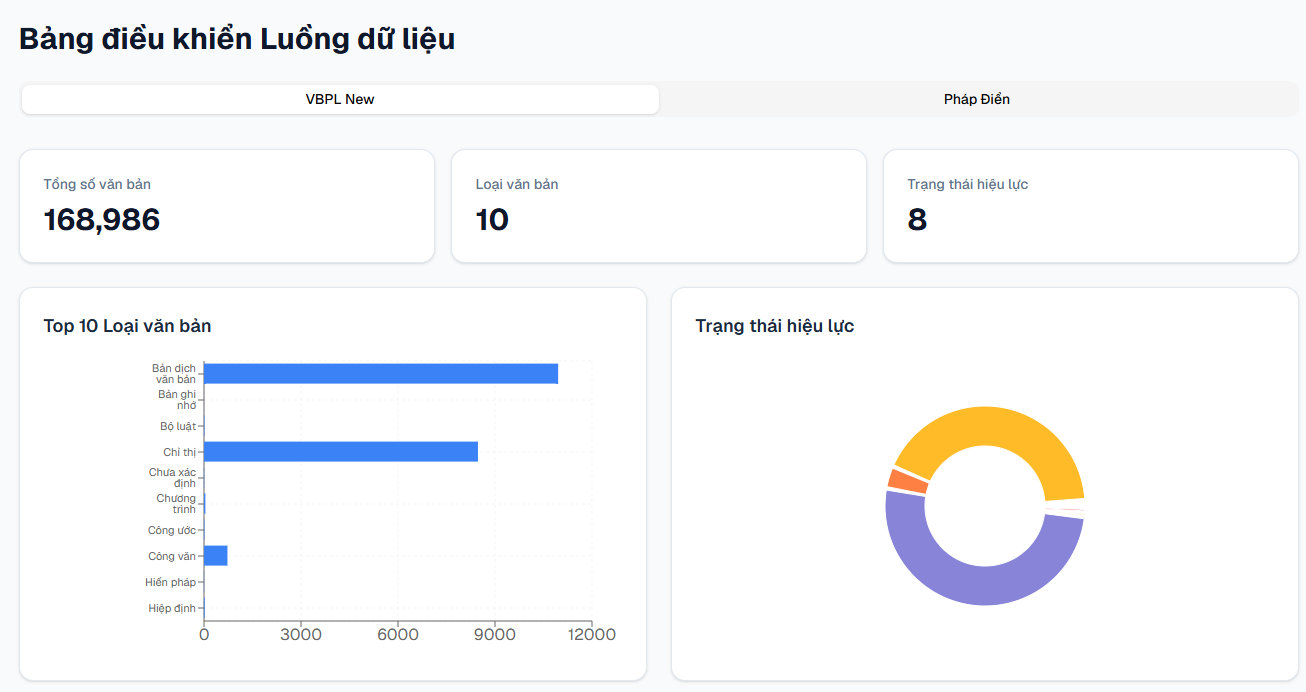
\includegraphics[width=0.99\textwidth]{pictures/WebUI/WebUI-AdminDataPipelineVbpl.png}
\caption{Giao diện đường ống dữ liệu VBPL}
\end{figure}

\begin{enumerate}
\item Quản trị viên mở trang đường ống dữ liệu VBPL.
\item Theo dõi trạng thái xử lý dữ liệu.
\item Kiểm tra tiến độ hoặc lỗi nếu có.
\end{enumerate}

\paragraph{Đường ống dữ liệu Pháp Điển}

\begin{figure}[H]
\centering
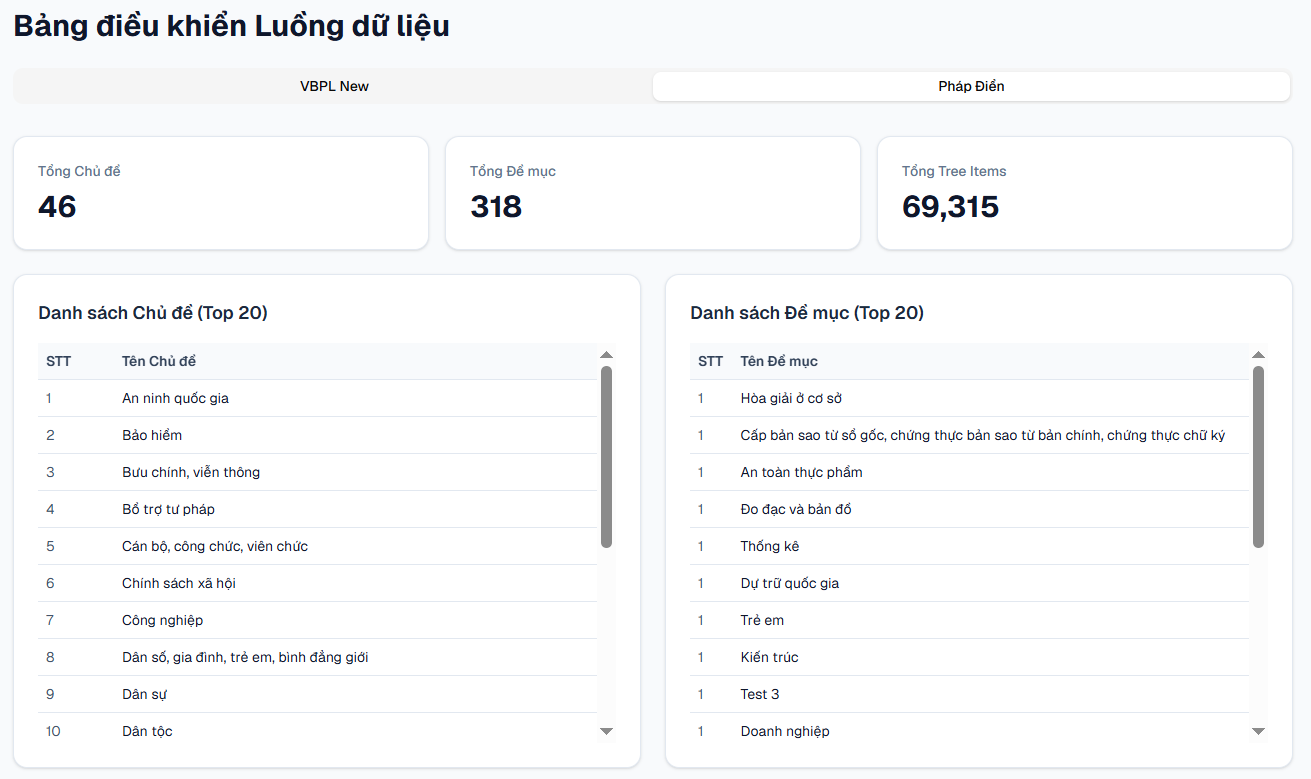
\includegraphics[width=0.92\textwidth]{pictures/WebUI/WebUI-AdminDataPipelinePhapDien.png}
\caption{Giao diện đường ống dữ liệu Pháp Điển}
\end{figure}

\begin{enumerate}
\item Quản trị viên mở trang đường ống Pháp Điển.
\item Xem thống kê cấu trúc và tiến độ xử lý.
\item Dùng thông tin này để theo dõi chất lượng dữ liệu.
\end{enumerate}

% \subsubsection{Thanh toán và gói VIP}

\paragraph{Danh sách gói thanh toán}

\begin{figure}[H]
\centering
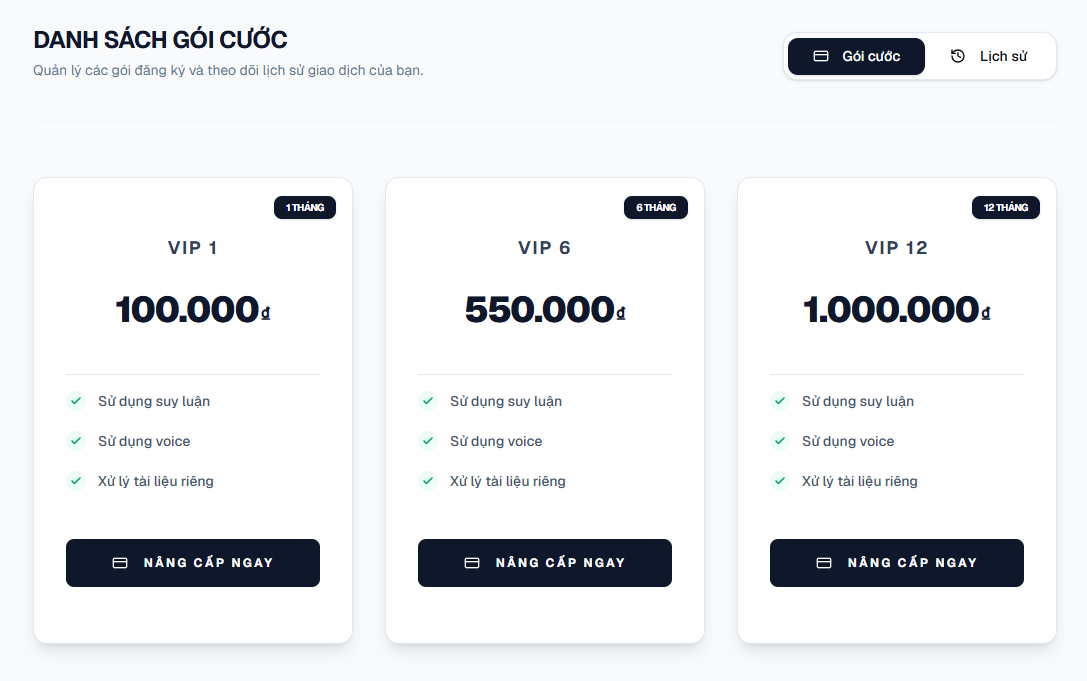
\includegraphics[width=0.92\textwidth]{pictures/WebUI/WebUI-PaymentPlanList.png}
\caption{Giao diện danh sách gói thanh toán}
\end{figure}

\begin{enumerate}
\item Người dùng mở trang gói VIP.
\item So sánh quyền lợi, giá và thời hạn từng gói.
\item Chọn gói phù hợp để tiến hành thanh toán.
\end{enumerate}

\paragraph{Lịch sử thanh toán}

\begin{figure}[H]
\centering
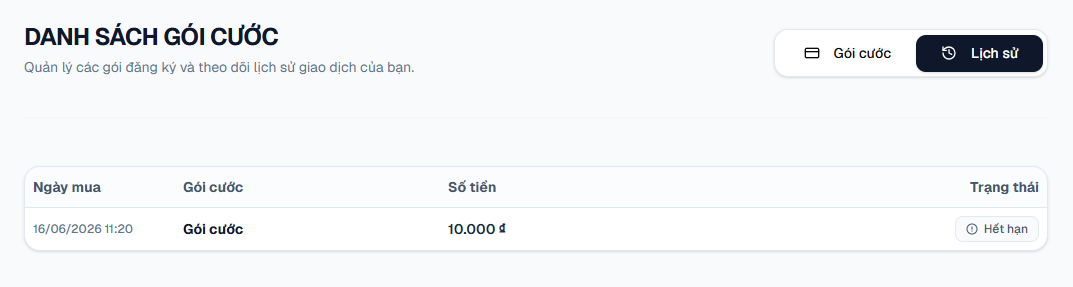
\includegraphics[width=0.92\textwidth]{pictures/WebUI/WebUI-PaymentHistory.png}
\caption{Giao diện lịch sử thanh toán}
\end{figure}

\begin{enumerate}
\item Mở trang lịch sử giao dịch.
\item Kiểm tra trạng thái, thời gian và gói đã thanh toán.
\item Dùng thông tin này để đối soát giao dịch khi cần.
\end{enumerate}

\paragraph{Thanh toán thành công}

\begin{figure}[H]
\centering
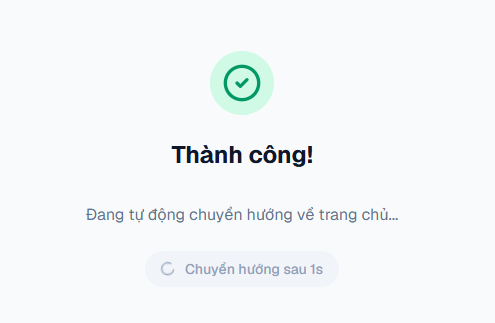
\includegraphics[width=0.5\textwidth]{pictures/WebUI/WebUI-PaymentSuccess.png}
\caption{Giao diện thanh toán thành công}
\end{figure}

\begin{enumerate}
\item Sau khi thanh toán, hệ thống hiển thị kết quả thành công.
\item Kiểm tra thông tin gói VIP vừa kích hoạt.
\item Quay lại hệ thống để sử dụng các tính năng VIP.
\end{enumerate}

\paragraph{Email thanh toán thành công}

\begin{figure}[H]
\centering
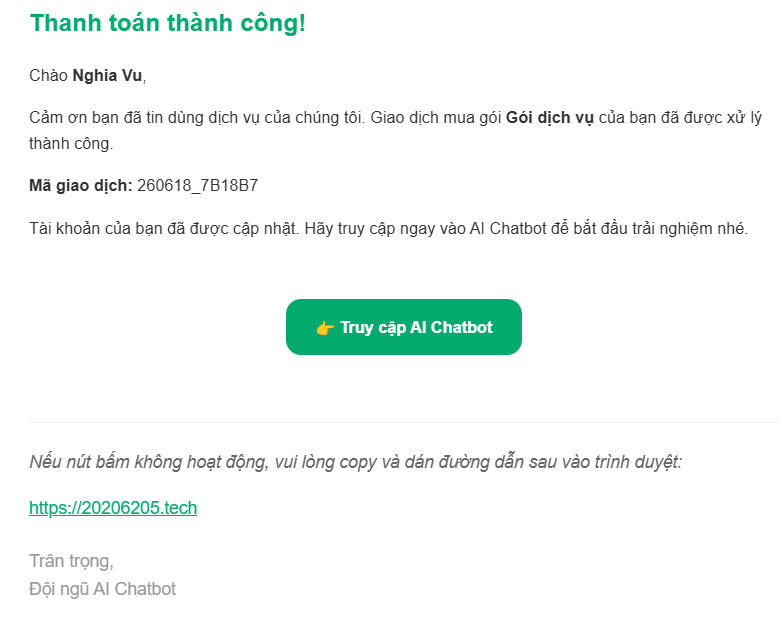
\includegraphics[width=0.6\textwidth]{pictures/WebUI/WebUI-PaymentSuccessEmail.png}
\caption{Giao diện email thanh toán thành công}
\end{figure}

\begin{enumerate}
\item Mở email thông báo thanh toán.
\item Kiểm tra thông tin gói, thời hạn và trạng thái giao dịch.
\item Lưu email để đối chiếu khi cần hỗ trợ.
\end{enumerate}

\paragraph{Gói VIP đang hoạt động}

\begin{figure}[H]
\centering
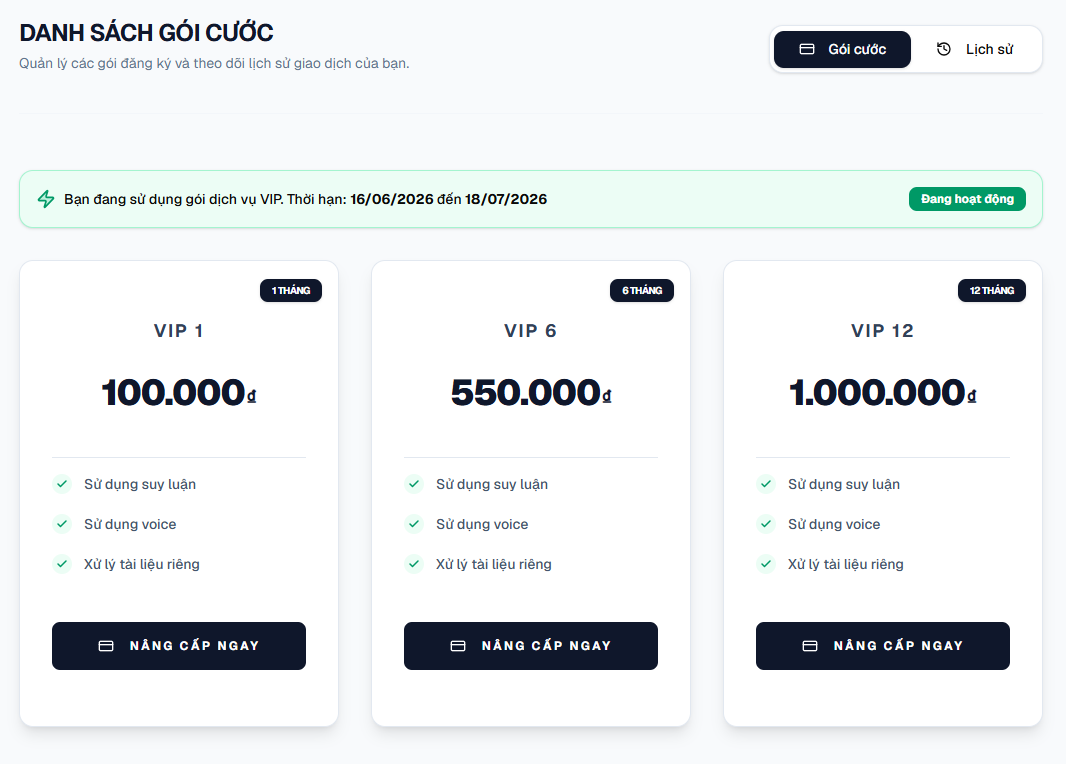
\includegraphics[width=0.92\textwidth]{pictures/WebUI/WebUI-PaymentPlanActive.png}
\caption{Giao diện gói VIP đang hoạt động}
\end{figure}

\begin{enumerate}
\item Mở trang gói VIP sau khi thanh toán.
\item Kiểm tra dấu hiệu gói đang hoạt động.
\item Sử dụng các tính năng yêu cầu VIP như suy luận, trò chuyện bằng giọng nói hoặc tài liệu cá nhân.
\end{enumerate}

% \subsubsection{Trò chuyện bằng giọng nói}

\paragraph{Chọn giọng nói}

\begin{figure}[H]
\centering
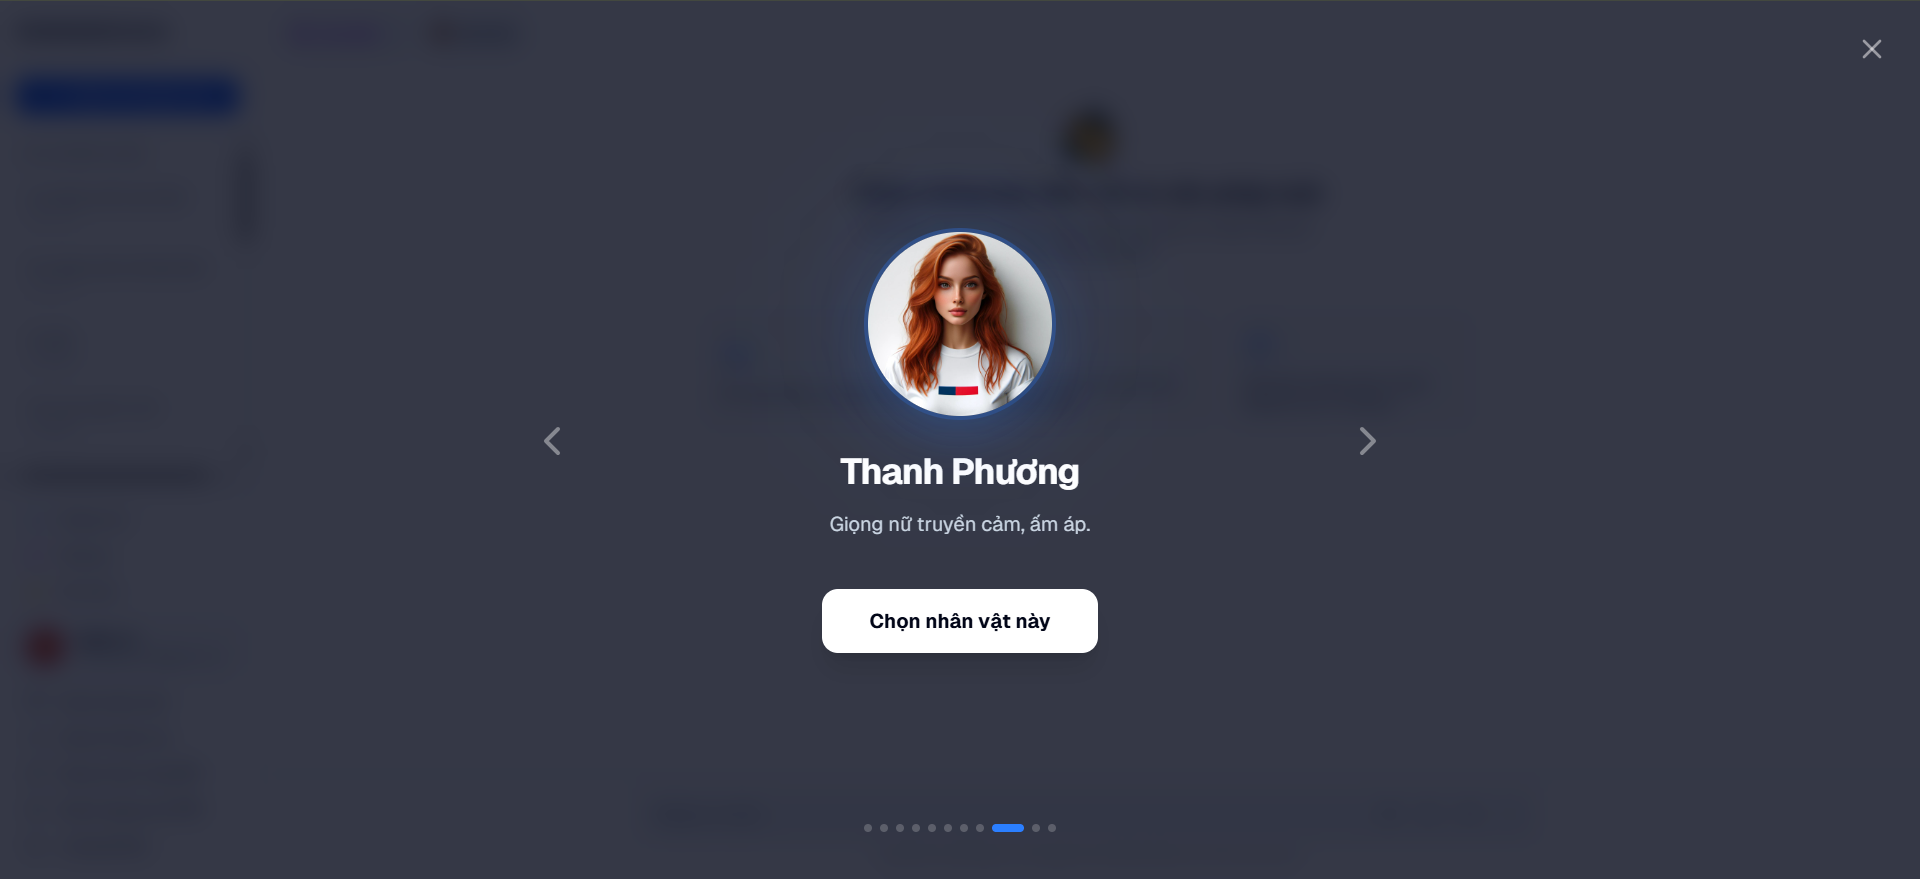
\includegraphics[width=0.92\textwidth]{pictures/WebUI/WebUI-VoiceSelect.png}
\caption{Giao diện chọn giọng nói}
\end{figure}

\begin{enumerate}
\item Mở phần chọn giọng nói hoặc nhân vật.
\item Nghe thử hoặc xem thông tin từng giọng.
\item Chọn giọng phù hợp cho cuộc trò chuyện.
\end{enumerate}

\paragraph{Trò chuyện bằng giọng nói}

\begin{figure}[H]
\centering
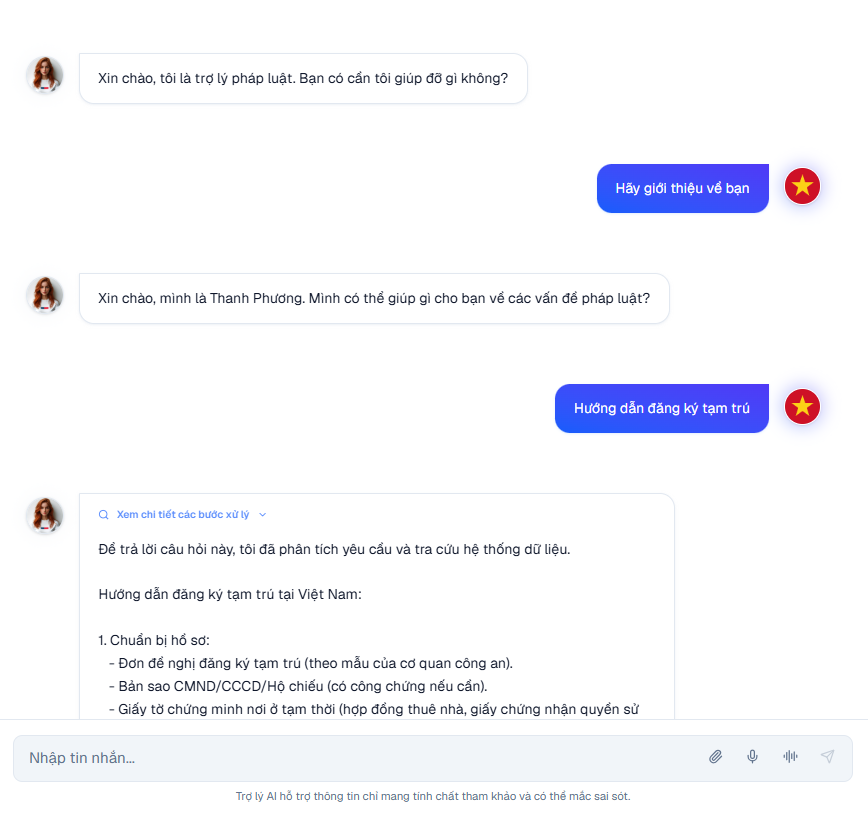
\includegraphics[width=0.92\textwidth]{pictures/WebUI/WebUI-VoiceChat.png}
\caption{Giao diện trò chuyện bằng giọng nói}
\end{figure}

\begin{enumerate}
\item Bắt đầu cuộc trò chuyện bằng giọng nói.
\item Nói câu hỏi hoặc yêu cầu vào micro.
\item Nghe phản hồi bằng giọng nói và theo dõi trạng thái xử lý trên giao diện.
\end{enumerate}

% \subsubsection{Tài liệu cá nhân}

\paragraph{Tải lên tài liệu}

\begin{figure}[H]
\centering
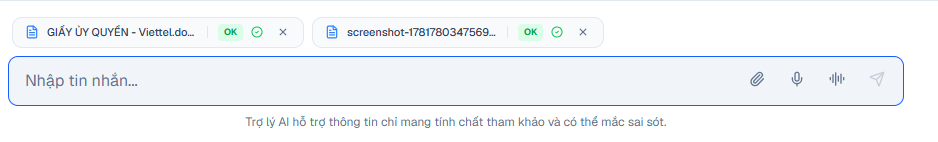
\includegraphics[width=0.92\textwidth]{pictures/WebUI/WebUI-DocumentUpload.png}
\caption{Giao diện tải lên tài liệu}
\end{figure}

\begin{enumerate}
\item Chọn file tài liệu từ thiết bị.
\item Bấm tải lên.
\item Chờ hệ thống xử lý nền trước khi dùng tài liệu trong trò chuyện.
\end{enumerate}

\paragraph{Trò chuyện với tài liệu}

\begin{figure}[H]
\centering
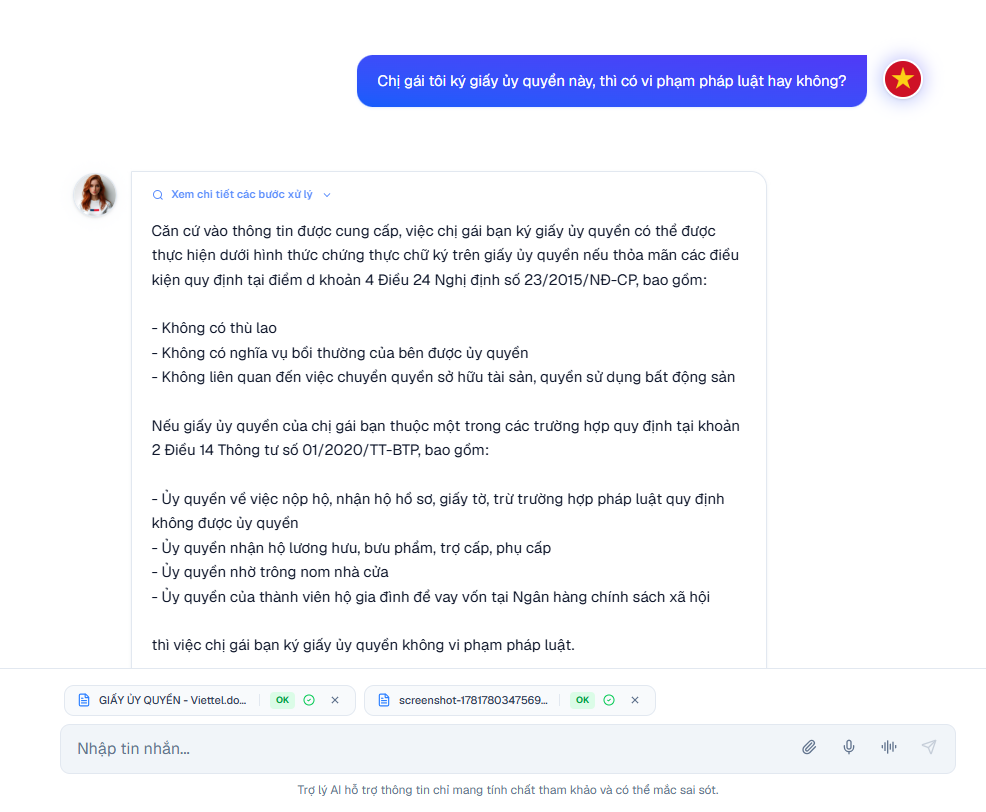
\includegraphics[width=0.92\textwidth]{pictures/WebUI/WebUI-DocumentChat.png}
\caption{Giao diện trò chuyện với tài liệu}
\end{figure}

\begin{enumerate}
\item Chọn tài liệu đã xử lý thành công.
\item Đặt câu hỏi liên quan đến nội dung tài liệu.
\item Xem câu trả lời và nguồn tham chiếu do hệ thống trả về.
\end{enumerate}
